% Chapter Template

\chapter{Efficacy Transition Pathways} % Main chapter title

\label{etp} % For referencing this chapter elsewhere, use \ref{etp}

%----------------------------------------------------------------------------------------
%	SECTION 1
%----------------------------------------------------------------------------------------

\section{Introduction}
\label{etp:Introduction}

In Phase \RN{2} trials we are often attempting to determine whether or not a new treatment or intervention works and establish if there is a efficacy signal. More specifically they aim to determine if there is sufficient level of evidence to warrant further research in a Phase \RN{3} setting \cite{jungRandomizedPhaseII2014}. In addition to assessing efficacy there is also opportunity to further explore the toxicity profile of the treatment compared to Phase \RN{1} trials Phase \RN{2} trials are typically conducted using a larger sample size \cite{evansFundamentalsClinicalTrial2010}. Generally speaking Phase \RN{2} trials should be efficient and quick such that we can progress to Phase \RN{3} as quickly as possible or drop any ineffective treatments.

The output from a Phase \RN{2} trial should be either a 'GO' or 'No GO' decision i.e should we or should we not proceed to later phase testing based on the data observed in this trial. One of the more important aspects of these trials is that we don't want to make any incorrect decisions and if there is an effective treatment that is being investigated we want to make sure that it is taken forward into Phase \RN{3}. As such it is important that we try to make correct decisions in Phase \RN{2} trials. Failure to do so could result in potentially beneficial treatments being rejected or bad treatments being investigated further, which could negatively impact patients and waste a lot of time and money \cite{vanPhaseIITrials2019}. 

However, Phase \RN{2} trials still face some issues which may make this challenging. Whilst it is the case that Phase \RN{2} trials are typically larger than Phase \RN{1} trials there are still some instances in which we would be dealing with small sample sizes. For example, in a rare disease setting. In these instances we may employ single arm Phase \RN{2} trial designs along with Bayesian methods to make better use of the data we are able to collect. 

Furthermore, we may also be interested in taking a look at the data more frequently to ensure the treatment is adequately safe and if there is some signal of efficacy to warrant continuing the trial. This may take the form of interim analyses and can be thought of in a similar manner to dose decisions in dose-finding trials. Rather than assessing the data and selecting a dose we are assessing if the trial should continue or not, stopping for either futility or safety reasons.  

Whilst these designs may be simple to implement they also suffer from similar drawbacks as certain dose-finding methodologies, that have previously been discussed. There may be some issues parametrising these designs e.g. selecting adequate decision rules. Any Bayesian approaches may be less familiar than traditional frequentist approaches that are more commonly used \cite{ivanovaNineyearChangeStatistical2016}, such as the Simon's two-stage design \cite{simonOptimalTwostageDesigns1989}. Clinicians and non-statisticians may struggle to understand why certain decisions are being made during interim and final analyses. 

In order to solve some of these issues Lucinda Billingham (LB) developed Efficacy Transition Pathways (ETPs) a novel visualisation tool to aid the design and interpretation of these types of designs. ETPs are an extension on the idea of Dose Transition Pathways (DTPs). Here they help map out and visualise the different decisions that can be made at interim and final analyses based on different observed outcomes in a similar manner as how DTPs present different dose-decisions that can be made for each cohort. 

In this chapter we will detail how ETPs are constructed as well as how they may be used in practice. In addition we present motivating examples where ETPs have been actively implemented and used in clinical trials. We then move on to the primary aim of this chapter which is to develop software around ETPs in order to make them accessible and as easy to implement as DTPs. 

%----------------------------------------------------------------------------------------
%	SECTION 2
%----------------------------------------------------------------------------------------

\section{Efficacy Transition Pathways}
\label{etp:ETPs}

ETPs were primarily designed for use in single arm Phase \RN{2} trials using Bayesian methods where the data is being looked at and assessed frequently. Typically a trial like this, at least in an oncology setting, will have a short-term binary outcome either success or failure, response or no response as its primary outcome. 

One approach for these sorts of trials is to use a Beta-Binomial conjugate analysis to estimate a response rate for the binary outcome. Posterior probabilities can be used to inform decision making and predictive probabilities can be used during interim analyses in a similar manner. Any decisions made will be done using pre-specified decision rules.

In order to demonstrate how ETPs are constructed and used we will look at the design process for a trial using a Beta-Binomial conjugate analysis. When implementing a design like this we need to consider a number of factors such as: the total sample size, the number and timing of any interim analyses, and decision criteria for interim and final analyses. Then much like with a dose-finding trial simulations can be conducted to obtain operating characteristics of the design. In addition we can also calculate the number of responses required at each analysis to continue the trial. This is also an iterative process so the design and decision rules can then be tweaked until an acceptable design is reached. 

ETPs can be utilised during this process as they are able to present the decisions that will be made based on the current design specification and the potential outcomes that can be observed for each analysis time point. As the design process for a trial involves multiple stakeholders it may not be easy to understand why or when certain decisions are being made. By mapping this all out in a single plot it may be easier to visualise. 

For example, based on whatever the current specification is, it may be the case that in the first interim analysis 2/5 patients require a response to continue the trial. Once the clinicians see this they may feel its too strict and would only think about stopping if there are no responses or alternatively they may want to remove this interim analysis and decide to only look at the data once 10 patients have been recruited. This is far more intuitive then trying to explain these concepts and using different boundaries for predictive probabilities. This could then be used to facilitate further discussions about the design specification and if decision rules need to be more or less lenient.  

ETPs much like DTPs could also be used throughout the trial as well. So, based on how many responses have already been observed you can easily figure out how many responses would be required for the next cohort of patients to obtain a 'GO' decision. Once the ETPs are produced all future decisions based on the number of responses can also be seen. So, this has the benefit of not requiring a statistician to run an analysis every time you need to figure out how many more responses are required for a 'GO' or 'No GO' decision. Whilst, ETPs should not replace the need for a statistician and they should still be involved with all the analyses they act as a tool that can help monitor the progress of a trial and can be referred to throughout the trials life cycle. In the next sections we provide an example trial to show how ETPs are constructed and utilised. 

%-----------------------------------
%	SUBSECTION 1
%-----------------------------------

\subsection{Illustrative example to showcase a Beta-Binomial design} 
\label{etp:BBIllEx}

Consider a Phase \RN{2} trial in which we are trying to evaluate the efficacy of some new treatment.This will be done using an outcome measure of response. Patients can either be considered a responder or a non-responder. Lets assume this is in a rare disease setting so patient numbers are limited and as such we will be using a single-arm design. The treatment effect will be the response rate and will be analysed using a Beta-Binomial conjugate model. We will require a sufficient level of evidence that the there is adequate treatment effect to warrant further research in a Phase \RN{3} trial.

To conduct the analysis and make a GO or No GO decision a prior and decision criteria need to be specified. For simplicity a minimally informative Beta(1,1) prior will be used. This represents a 50\% response rate from a group of two patients. Data will also need to be collected from patients recording if they had a response or not. This in turn is combined with the prior distribution to generate a posterior distribution for the treatment effect. Then pre-specified rules based on these direct probabilities from the posterior can be used for decision making purposes. This can take the form of

\begin{equation}
	\label{eq_etp:betafinaldecrule}
	P(\theta > c |y) \geq q  \; \; \; \; \text{then GO else No GO}
\end{equation}

where $\theta$ is the treatment effect (response rate), $c$ is some target level of treatment effect (target response rate), $y$ represents our data and $q$ is some threshold of sufficient evidence (acceptable probability level). 
 
For our example the following decision rule will also be used $P(\theta  \geq 30\%) \geq 0.9$. So, if there is a greater than  90\% chance that the true response rate is at least 30\% this will be considered sufficient evidence to warrant a GO decision. We will also include interim analyses after every five patients to evaluate whether or not the trial should be stopped for futility. To do this we will use the predictive probability of success (PPoS).

This works by evaluating the data at pre-specified time points or after a certain number of patients have been recruited, in this example after every five patients. At these time points we can determine whether or not we have observed enough responses to warrant continuing with the trial based on the overall minimum responses we would need for a final GO decision. More explicitly the PPoS is the probability of the trial being considered a success given the current data observed at the interim analysis. This is calculated by predicting the future number of responses in the patients yet to be recruited based on the data that has already been observed and the prior distribution.

For our example trial we will specify a PPoS acceptable probability threshold where if PPoS < 0.05 then we should stop the trial for futility. This implies we would stop the trial if there is a less than 5\% chance that the response rate at the end of the trial will be greater than 30\% with a probability of 0.9 i.e a less than 5\% chance that the trial would reach a GO decision or be considered a success. 

Table \ref{tab_etp:exampleBBspecs} details the minimum number of responses required under this design at each analysis time point. For the final analysis, once 30 patients have been recruited, a minimum of 13 responses must be observed in order to have a GO decision. We can also see what the minimum number of responses required are for each interim analysis.

\begin{table}[h!]
	\centering
	\caption{Specification of parameters for the example Beta-Binomial trial.}
	\label{tab_etp:exampleBBspecs}
	\begin{tabular}{l|c}
		\hline
		\textbf{Analysis}     & \textbf{Minimum No. Responses for GO Decision}               \\ \hline
		N = 5  & 1                            \\
		N = 10 & 2                            \\
		N = 15 & 3                           \\
		N = 20 & 7                            \\
		N = 25 & 9                         \\
		N = 30 & 13                  \\ \hline
	\end{tabular}
\end{table}

Most of the specifications we have made here along with our decision rules are fairly arbitrary. In practice decision rules should be decided before the trial starts. This is typically done via the evaluation of simulations and looking at the minimum number of responses required for GO decisions. Multiple scenarios corresponding to different true response rates can be investigated. The probability of making a correct decision can then be calculated. This represents the power of our design. For scenarios with low true response rates (relative to the target response rate) we want the probability of making a No GO decision to be high. Similarly, for scenarios with high true response rates we want the probability of making a GO decision to be high. The decision rule parameters, the target response rate and probability threshold can then be adjusted to ensure the design is making appropriate decisions in these scenarios. 	

Whilst simulations are useful they may not convey what is most meaningful for other collaborators when assessing the merits of each iterative design specification. This is where ETPs can be used to try and bridge that gap by offering a way to visually represent key information and decisions that are made with these types of designs. In the next section we detail how an ETP is constructed using the example trial design specified here. 


%-----------------------------------
%	SUBSECTION 2
%-----------------------------------

\subsection{Constructing Efficacy Transition Pathways} 
\label{etp:conETPs}

At each interim analysis PPoS is calculated based on the number of responses observed thus far and evaluated to see if it meets the decision criteria. Therefore there will be a minimum number of responses that have to be observed in order to continue recruitment. This is similar to how we can calculate the number of responses required at the end of the trial to warrant a GO decision. Obviously, the minimum number of responses required at each interim and the final analysis depends on the decision criteria that is specified. 

Intuitively, it is easier to understand that three responses have to be observed from 15 patients rather than a PPoS $\leq 0.05$ is needed. Through discussions with clinicians we can then calibrate our decision criteria based on these interpretations. We may want to be more strict or lenient at our interim. If the clinicians would be happy to continue recruitment after seeing only two responses we could lower the PPoS threshold, likewise if they wanted to be confident and only continue if six responses were observed we would increase the PPoS threshold. Similarly, this can also be done for the final analysis decision criteria. The acceptable probability level or target response rate could be adjusted so a specific minimum number of responses observed achieves a GO decision. Obviously any changes made should be assessed by simulations as well, drastically changing the decision criteria could have a negative impact on performance. 
 
As you add more interims to a design like this trying to understand the break points at each interim become more complex. A solution for this is ETPs. In our example trial we have a maximum sample size of 30 patients with interim analyses planned after every five patients. This results in a total of six analyses, one final analysis and five interims. The decision criteria at the end of the trial requires the treatment effect to be greater than 30\% with a probability of 0.9 and to pass the interim analyses we require the PPoS to be greater than 0.05. 

To construct an ETP we produce individual cells which contain key information about a specific outcome i.e. a certain amount of responses. If we consider our first interim at five patients, at that point there are six different possible outcomes that can be observed. Either one, two, three, four or all five of the patients had a response or none of them did. For each possible outcome we can then calculate the PPoS as well as the Bayesian estimate of the response rate and an associated credible interval. Figure \ref{fig_etp:Cell0Resp5Pat} shows what this cell would look like. 

\begin{figure}[h!]
	\centering
	\caption{ETP cell plot for 0 responses in 5 patients.}
	\label{fig_etp:Cell0Resp5Pat}
	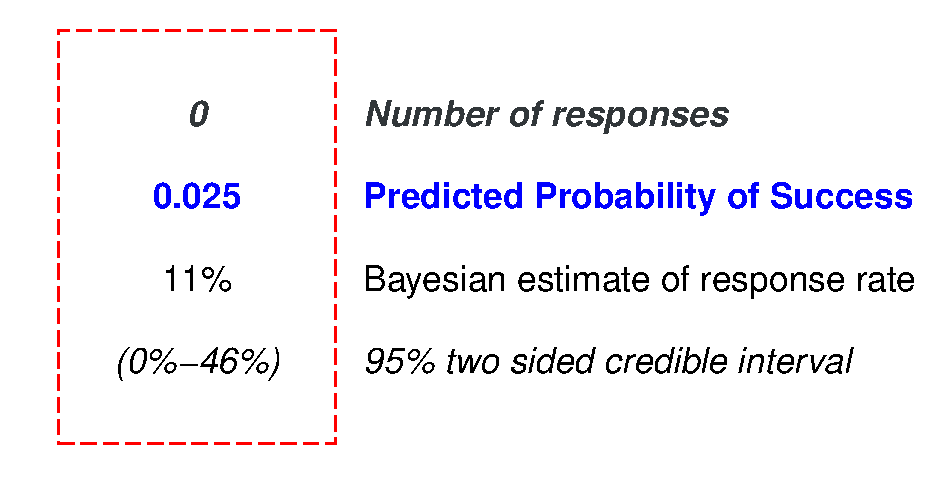
\includegraphics[width=\textwidth]{ETP-cell0Resp5Pat}
\end{figure}

The number at the top indicates the outcome for the cell, in this case the number of responses which is 0. The second row shows the PPoS in this scenario, the third row showing the Bayesian estimate of response rate and the last row shows the 95\% credible interval. For 0 responses the PPoS is 0.025 which is less than our threshold so the decision here would be to stop. This is represented by the red dashed line. From this one cell we are able to see what the decision would be at the interim analysis time point if this is the outcome that is observed. We are also able to see specifically what the PPoS and estimated response rate would be as well. The choice was made to present probabilities with decimals and any estimates of response rates with percentages. This was so the two could easily be differentiated and if you wanted to make a comment about the treatment effect we could directly look at the percentages and see the estimate and credible interval.   

Cells are generated for each possible outcome at each interim time point. Figure \ref{fig_etp:Cell2Resp5Pat} shows the cell for two responses in five patients. Here we can see the PPoS is 0.501 which is greater than our threshold so the decision would be made to continue recruitment. This is indicated by the green dashed line. As we put each cell together we can then clearly see the minimum number of responses required to continue recruiting.  

\begin{figure}[h!]
	\centering
	\caption{ETP cell plot for 2 responses in 5 patients.}
	\label{fig_etp:Cell2Resp5Pat}
	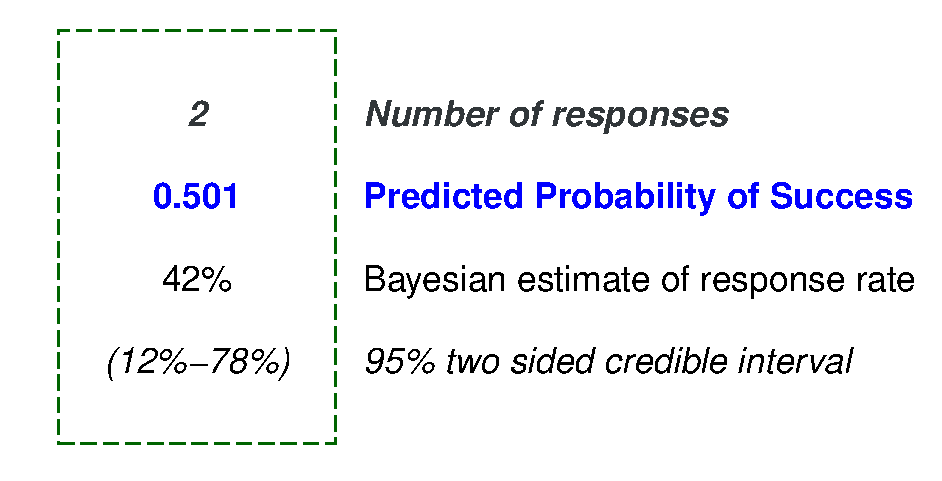
\includegraphics[width=\textwidth]{ETP-cell2Resp5Pat}
\end{figure}

This process is then repeated for each interim analysis. So, the next analysis would be at 10 patients. Here we would generate 11 cells for all the different possible outcomes (no response, one response, two responses, ..., 10 responses). The same would then be done for the analysis at 15, 20 and 25 patients. 

For the final analysis the presentation of the cells is slightly different. Here we are no longer interested in PPoS as no more patients will be recruited and rather we can just evaluate if the trial has met the decision criteria. So, in each cell rather than present PPoS the posterior probability that the response rate is greater than our target rate is presented instead. Figures \ref{fig_etp:Cell10Resp30Pat} and \ref{fig_etp:Cell14Resp30Pat} show the cells for 10 responses and 14 responses out of 30 patients respectively. In this example our $q$ is set at 0.9 so if the posterior probability is greater than that we have a GO decision. 

\begin{figure}[h!]
	\centering
	\caption{ETP cell plot for 10 responses in 30 patients.}
	\label{fig_etp:Cell10Resp30Pat}
	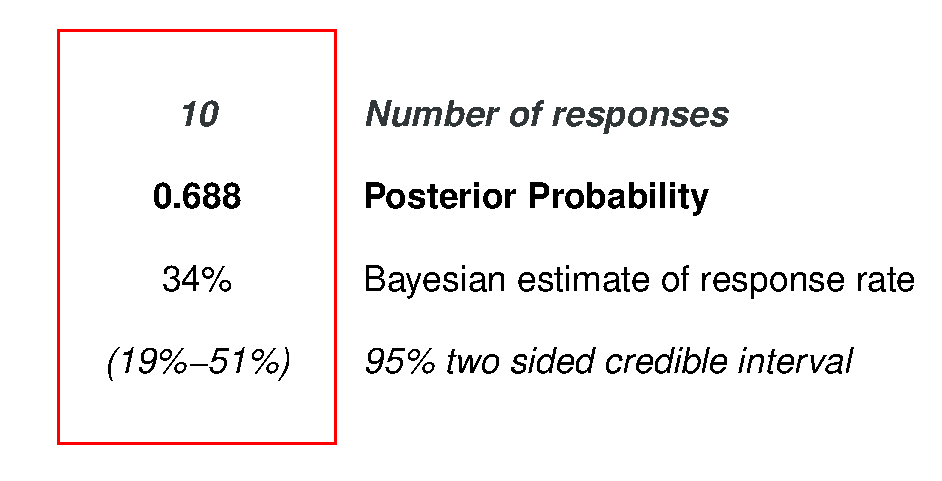
\includegraphics[width=\textwidth]{ETP-cell10Resp30Pat}
\end{figure}


\begin{figure}[h!]
	\centering
	\caption{ETP cell plot for 14 responses in 30 patients.}
	\label{fig_etp:Cell14Resp30Pat}
	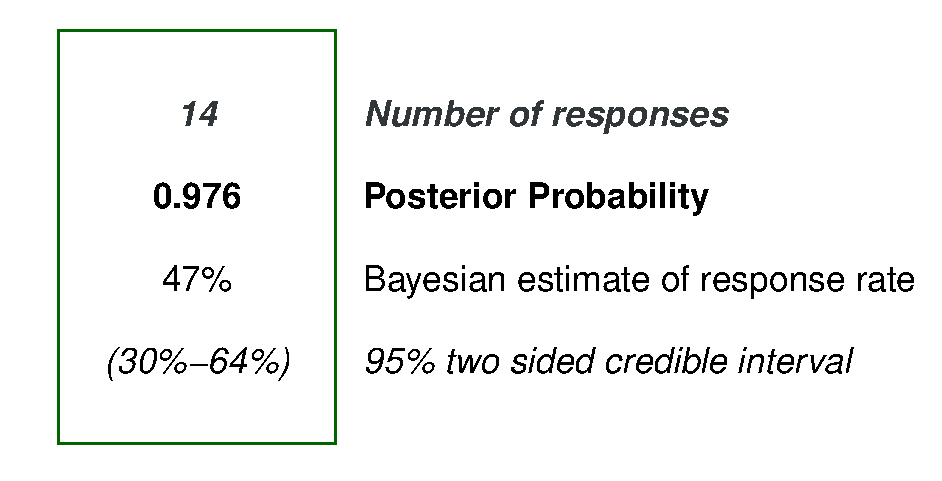
\includegraphics[width=\textwidth]{ETP-cell14Resp30Pat}
\end{figure}


The efficacy transition pathway is then constructed by grouping each cell for each interim analysis and then stacking those group of cells together. For our example trial the ETP is shown in Figure \ref{fig_etp:ConstructedETP}. Each row of cells in the ETP represents each interim analysis with the final row representing the final analysis. One adaptation made with the cells is that the confidence interval is presented across the bottom two rows in each cell just to make the figure easier to read and more scalable. 

From this figure what can clearly be seen is when we do or do not have a GO decision. At each interim of 5, 10, 15, 20, 25 patients we can see that the minimum number of responses for a GO decision is 1, 2, 4, 7 and 9 respectively. Also, for the final analysis a minimum of 13 responses is required. We can also read down the figure to gauge an idea of how many additional responses would be required in future analyses to warrant a GO decision. For instance if you observed five responses in your first cohort of five patients, that is enough observed data to continue passing the interim decision criteria until the fourth interim analysis in which case you would need an additional two responses. This can easily be seen by reformatting the ETP to be aligned to the left so the same number of responses are stacked on top of each other for each cohort. This is illustrated in Figure \ref{fig_etp:ConstructedETPleft}. 

In addition to the easy visualisation of the number of responses required to achieve a GO decision we can also quite easily see the estimates of the treatment effect for each potential outcome and each analysis time point. This is useful for interpreting the results for the final analysis (the bottom row of the ETP plot). Right away from interpreting the cell for the minimum number of responses (13/30) for a GO decision we can see the estimated response rate would be 44\% with a probability of 0.95 that the true response rate is between 27\% and 61\%. We also need to keep in mind the original decision rule for the final analysis which for any GO decision implies there is a greater than 0.9 probability that the response rate is greater than 30\%. This can then be used to facilitate discussions with the clinicians to deem if this is an acceptable level of evidence to warrant further research or potentially bring into practice, based on previous studies, current treatments or their experience. We can then adjust our design and decision rules accordingly, which we discuss in the next section. 

\begin{sidewaysfigure}
	\centering
	\caption{Example of a constructed ETP.}
	\label{fig_etp:ConstructedETP}
	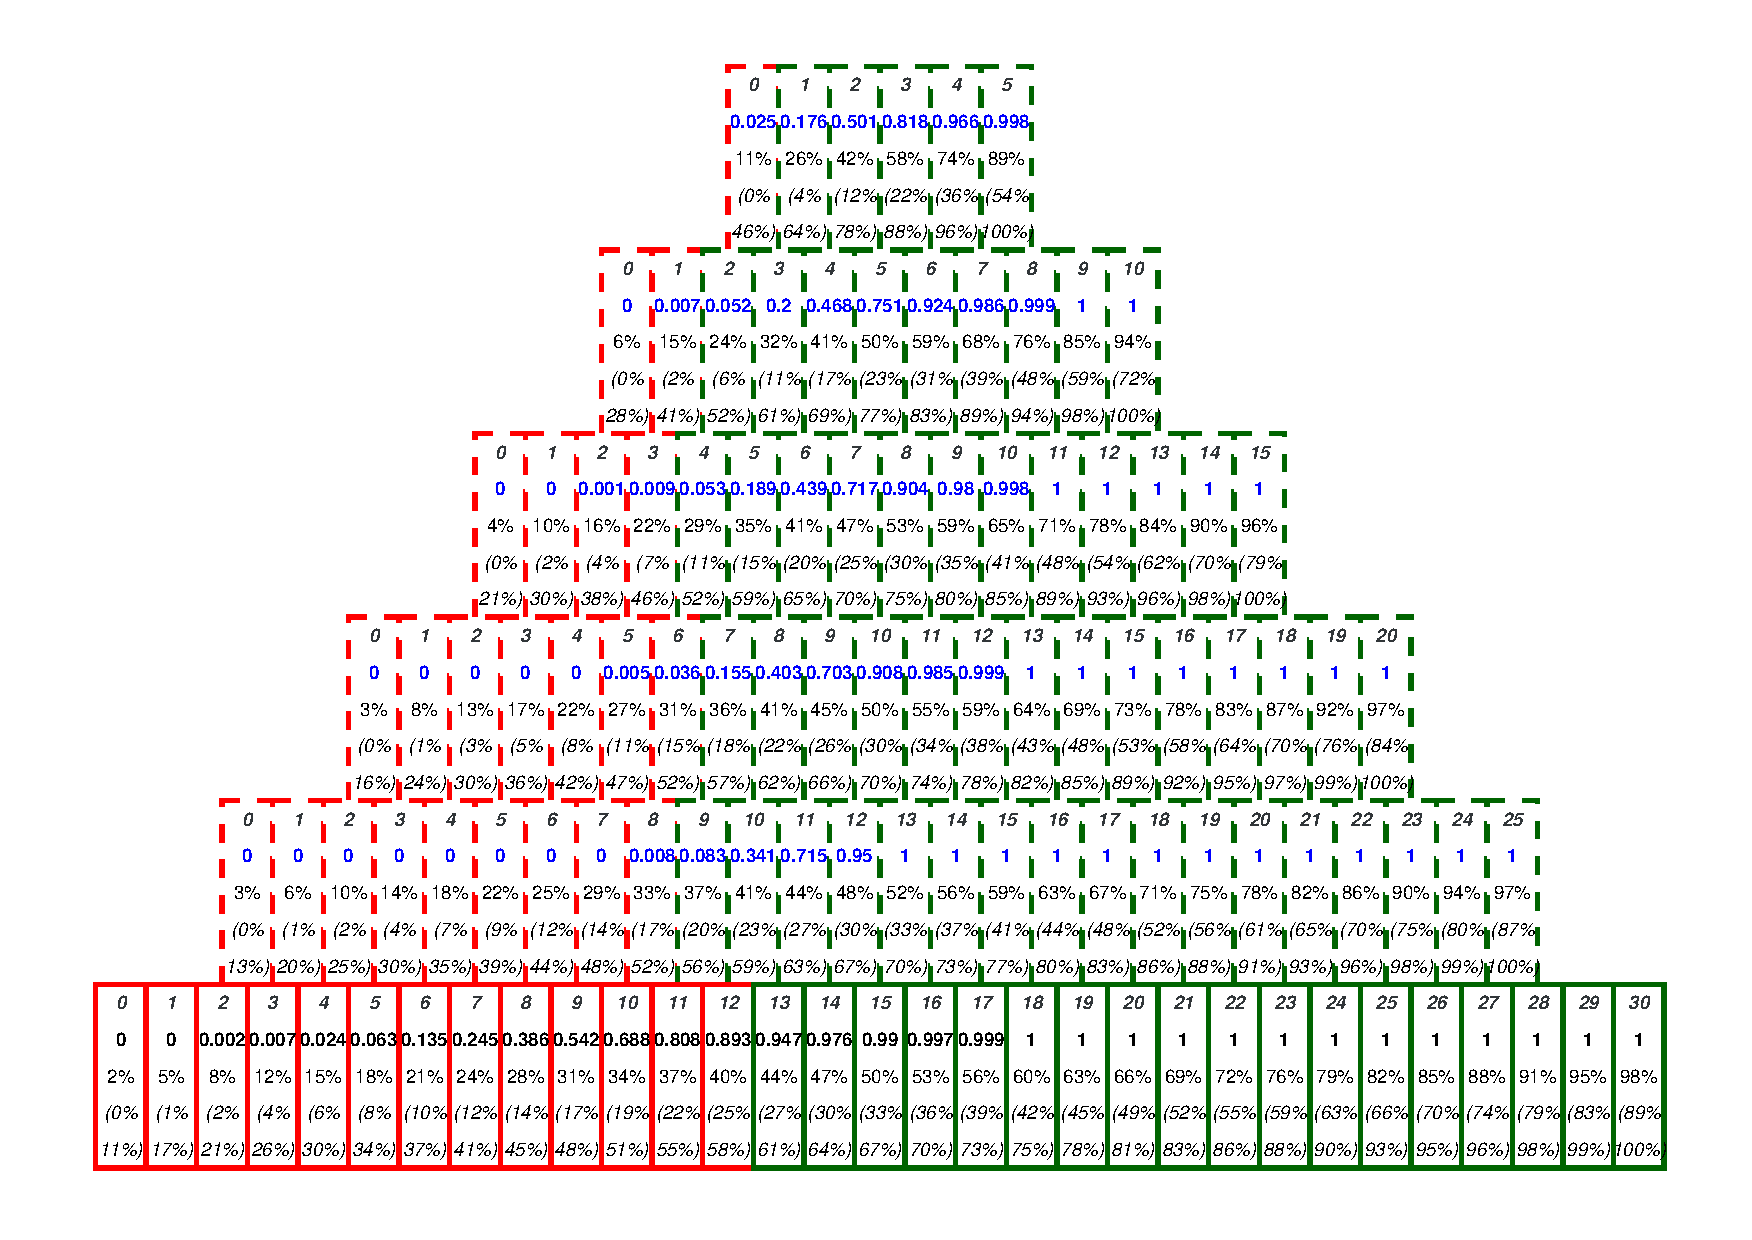
\includegraphics[width=25cm, height=15cm]{ETP-constructed}
\end{sidewaysfigure}

\begin{sidewaysfigure}
	\centering
	\caption{A left aligned version of the constructed ETP.}
	\label{fig_etp:ConstructedETPleft}
	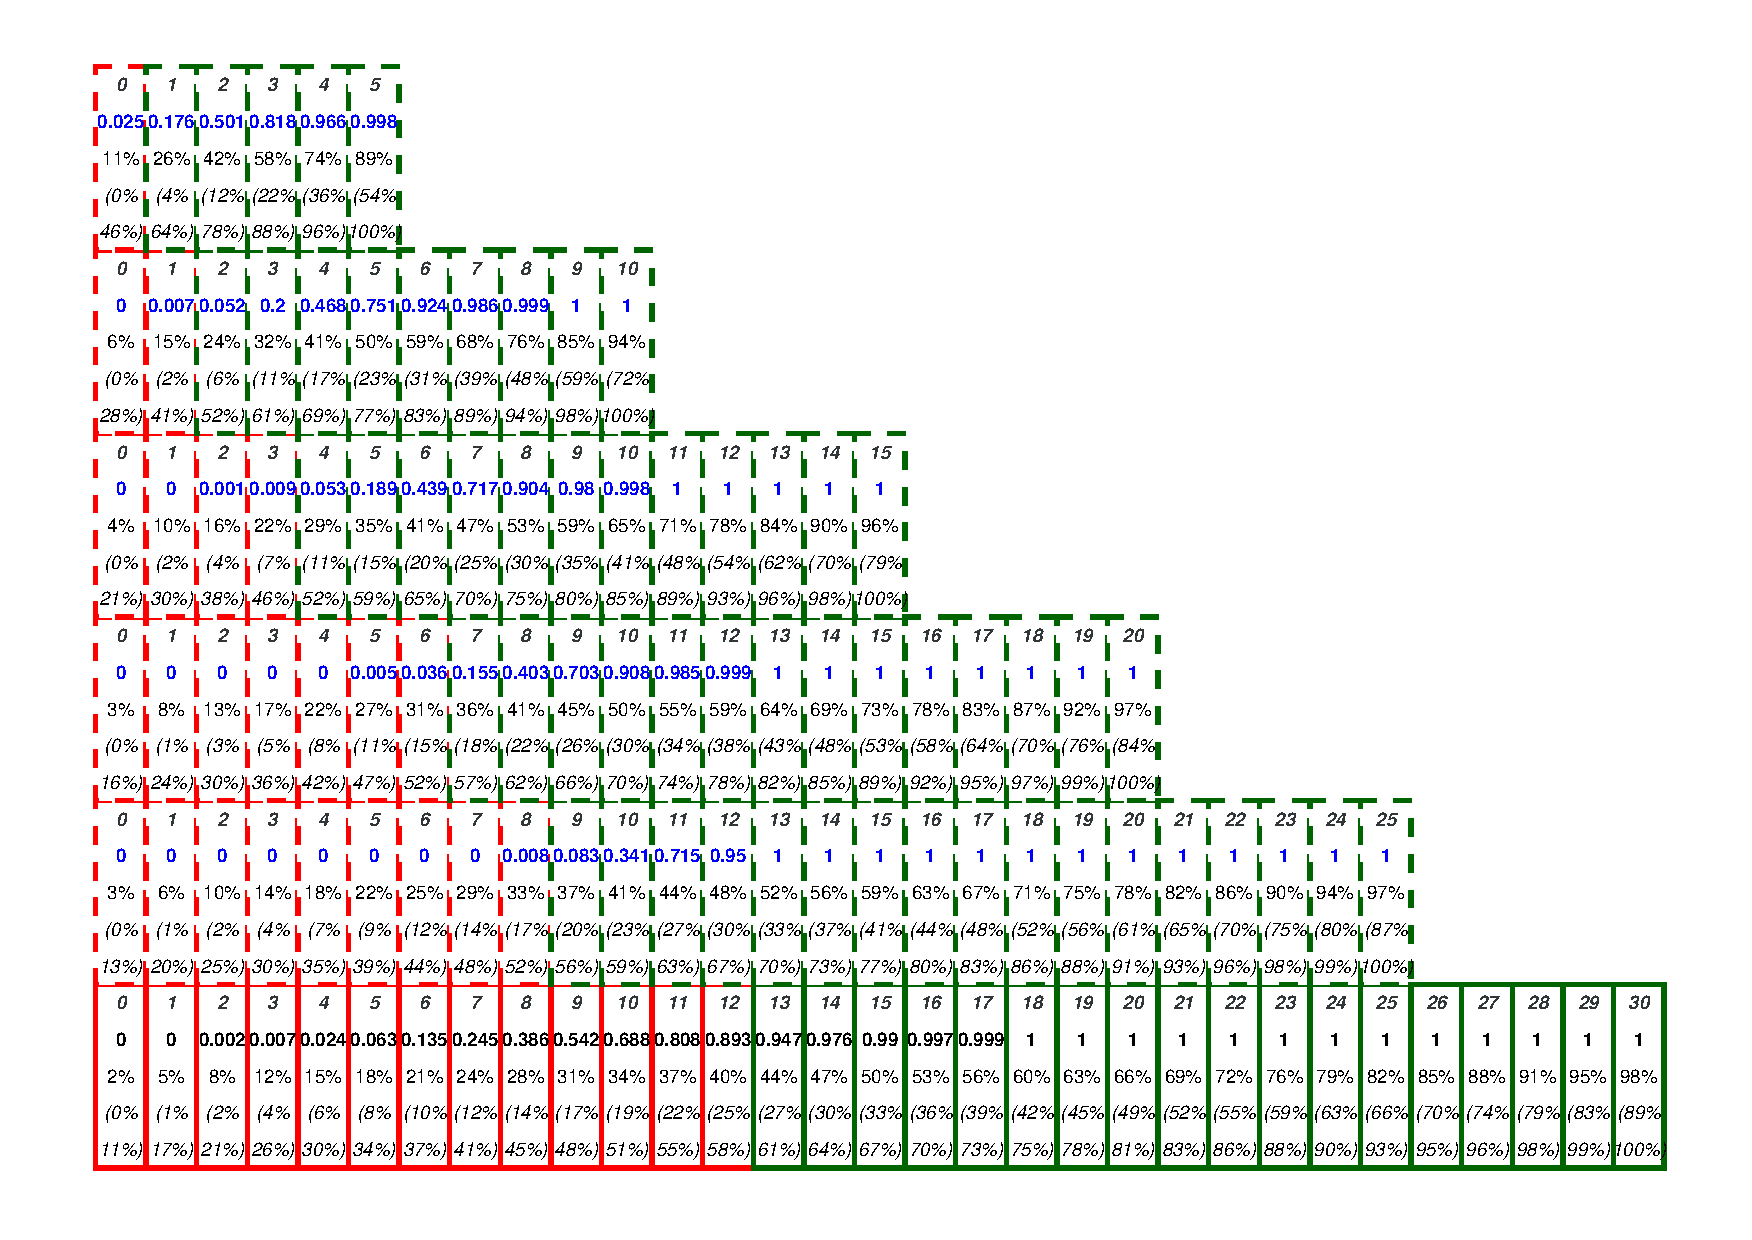
\includegraphics[width=25cm, height=15cm]{ETP-constructedleft}
\end{sidewaysfigure}

\newpage
%-----------------------------------
%	SUBSECTION 3
%-----------------------------------

\subsection{Updating decision criteria based on Efficacy Transition Pathways} 
\label{etp:updatingETPs}

Having seen the ETP we created for our example trial, suppose we want to modify our decision criteria such that a GO decision at the final analysis requires only nine patients to achieve a response. Compared to the initial decision criteria, which required 13 responses, we may want to  consider lowering this due to the treatment options available for these patients may not being very effective. Obviously there may be many reasons why we would want to increase or decrease this requirement and this would depend on the context and background of each individual trial. This is just to provide an illustrative example of why we might consider changing the criteria and how we go about it with ETPs. 

By looking directly at the ETP Figures \ref{fig_etp:ConstructedETP} or \ref{fig_etp:ConstructedETPleft} we can see that nine responses out of 30 patients has a posterior probability of 0.542. So, based of the initial decision rule of $P(\theta  \geq 30\%) \geq 0.9$, this implies that the probability that the response rate is greater than or equal to 30\% is 0.542. Therefore, if we wanted to make this a GO decision we would change our decision criteria such that our acceptable level of probability was something smaller than that posterior probability. For example, a new decision rule could be $P(\theta  \geq 30\%) \geq 0.5$ this would mean that nine responses out of 30 patients would now be a GO decision. This is another benefit of ETPs, we can quickly ascertain how we would need to change our decision criteria to be in order for a specific minimum number of responses to be a GO decision. 

Let's say we implement that new decision rule, we can then create an updated ETP. In Figure \ref{fig_etp:ConstructedETP_30-50_5} we can see for the final analysis (the bottom row of the plot) GO decisions start from nine responses. It is important to note the content of these cells haven't changed. The estimates of response rates and credible intervals are still the same. This is because we fundamentally haven't made any changes to the design just the criteria for which we are making decisions. Changes in these estimates would only be triggered if we were to change the total sample size. Additionally the posterior probabilities are also consistent with the previous ETP, this is because we haven't altered the targeted response rate in our decision criteria. This value is still showing the probability that the treatment has a response rate greater than 30\%. These values would only differ if our target response rate was set as something else. For the rest of the cells showing previous cohorts and the interim analyses we can see the minimum number of responses required for a GO decision is now 0, 1, 3, 4 and 6 for each interim analysis respectively. Also, note how the PPoS is different compared to the last ETP this is because PPoS takes into account the final decision rule we are using. Any change to that rule will impact PPoS calculations. 

\begin{sidewaysfigure}
	\centering
	\caption{ETP with updated final decision rule.}
	\label{fig_etp:ConstructedETP_30-50_5}
	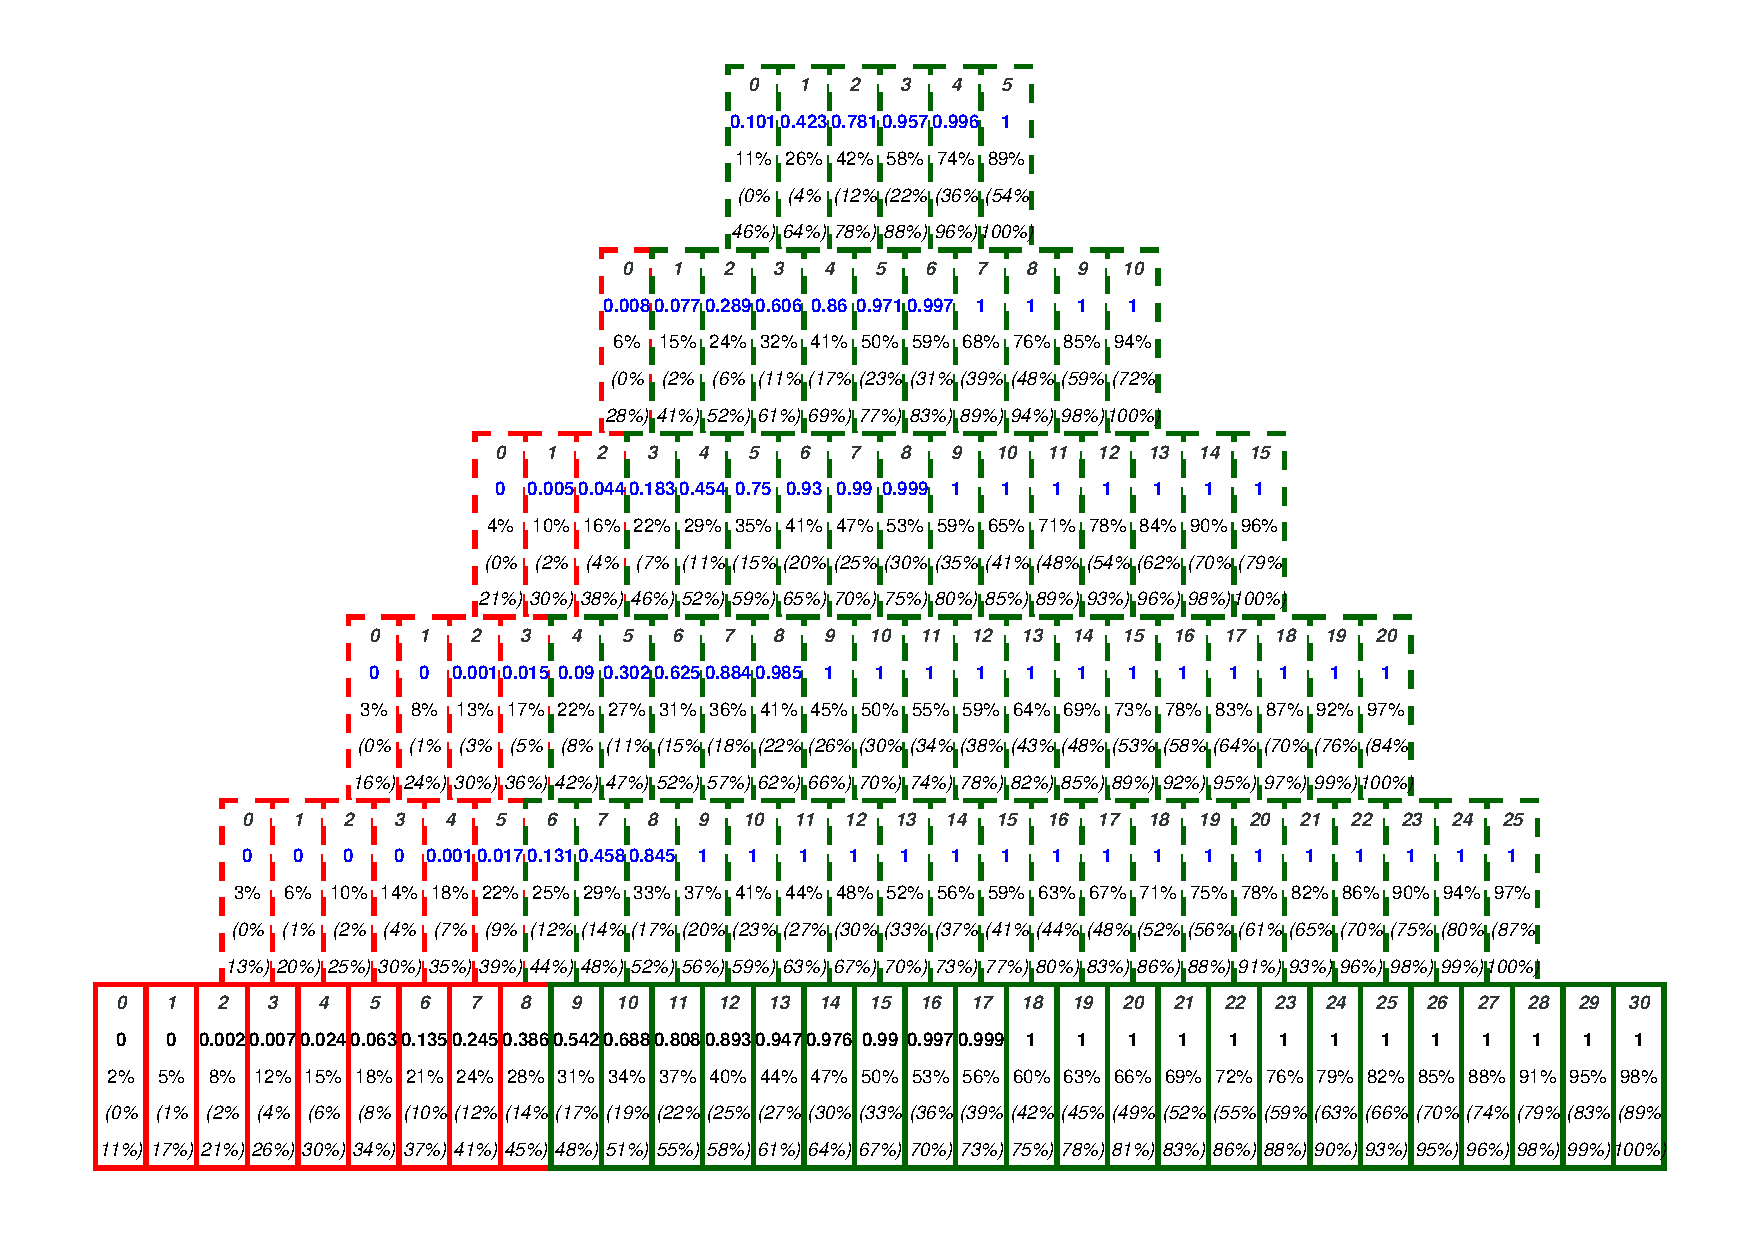
\includegraphics[width=25cm, height=15cm]{ETP-constructed_30-50_5}
\end{sidewaysfigure}

By altering our decision rule like this we ensure that if we observe the desired number of responses, in this case nine, the trial would be a success. We did this by just changing $q$, the acceptable probability level. However, it should be noted that this can also be achieved by changing both $c$ (the target response rate) and $q$. These values can both be manipulated so we still maintain the same practical decision making. This is important to note as whilst clinicians may find it more intuitive to specify decision rules based on a minimum number of responses there are different ways in which that can be achieved. 

Table \ref{tab_etp:DecisionCriteria} details the posterior probability that the estimated response rate is greater than four different target response rates given we observe nine responses out of 30 patients. If our target response rate is 10\% and we observe nine responses the posterior probability is 0.999 so then our decision rule can be specified as if $P(\theta  \geq 10\%) \geq 0.95$. Here our value of $q$ just has to take a value lower than the posterior probability but we should be careful to make sure it isn't low enough such that observing 8 responses also becomes a GO decision. We can then make similar statements about the other target response rates presented in the table. The associated decision criteria for those response rates are also presented. 

\begin{table}[h!]
	\centering
	\caption{Examples of different decision criteria.}
	\label{tab_etp:DecisionCriteria}
	\begin{tabular}{c|c|c}
		\hline
		\textbf{Posterior Probability for 9 Responses}     & \textbf{$c$}  & \textbf{$q$}              \\ \hline
		$P(\theta  \geq 10\%) =  0.999$  & 10\% 	& 0.95                            					\\
		$P(\theta  \geq 20\%) =  0.926$  & 20\%     & 0.90                         \\
		$P(\theta  \geq 30\%) =  0.542$  & 30\%     & 0.50                      \\
		$P(\theta  \geq 40\%) =  0.143$  & 40\%     & 0.10                    \\ \hline
	\end{tabular}
\end{table}

This is also shown in Figure \ref{fig_etp:DecisionCriteria}.  Here there are four curves each representing the posterior probability that the estimated response rate is greater than the target response rates of 10\%, 20\%, 30\% and 40\% for all possible number of responses. The dashed vertical line represents the minimum number of responses we would require for a GO decision. Where the dashed like intercepts with each curve is posterior probability that the treatment effect is greater than those target response rates and should be used to inform our values of $q$. By adding in more curves for different target response rates or moving the dashed like for a different number of minimum responses we can determine appropriate values for our decision criteria. 

\begin{figure}[h!]
	\centering
	\caption{Changes in posterior probability for decision criteria.}
	\label{fig_etp:DecisionCriteria}
	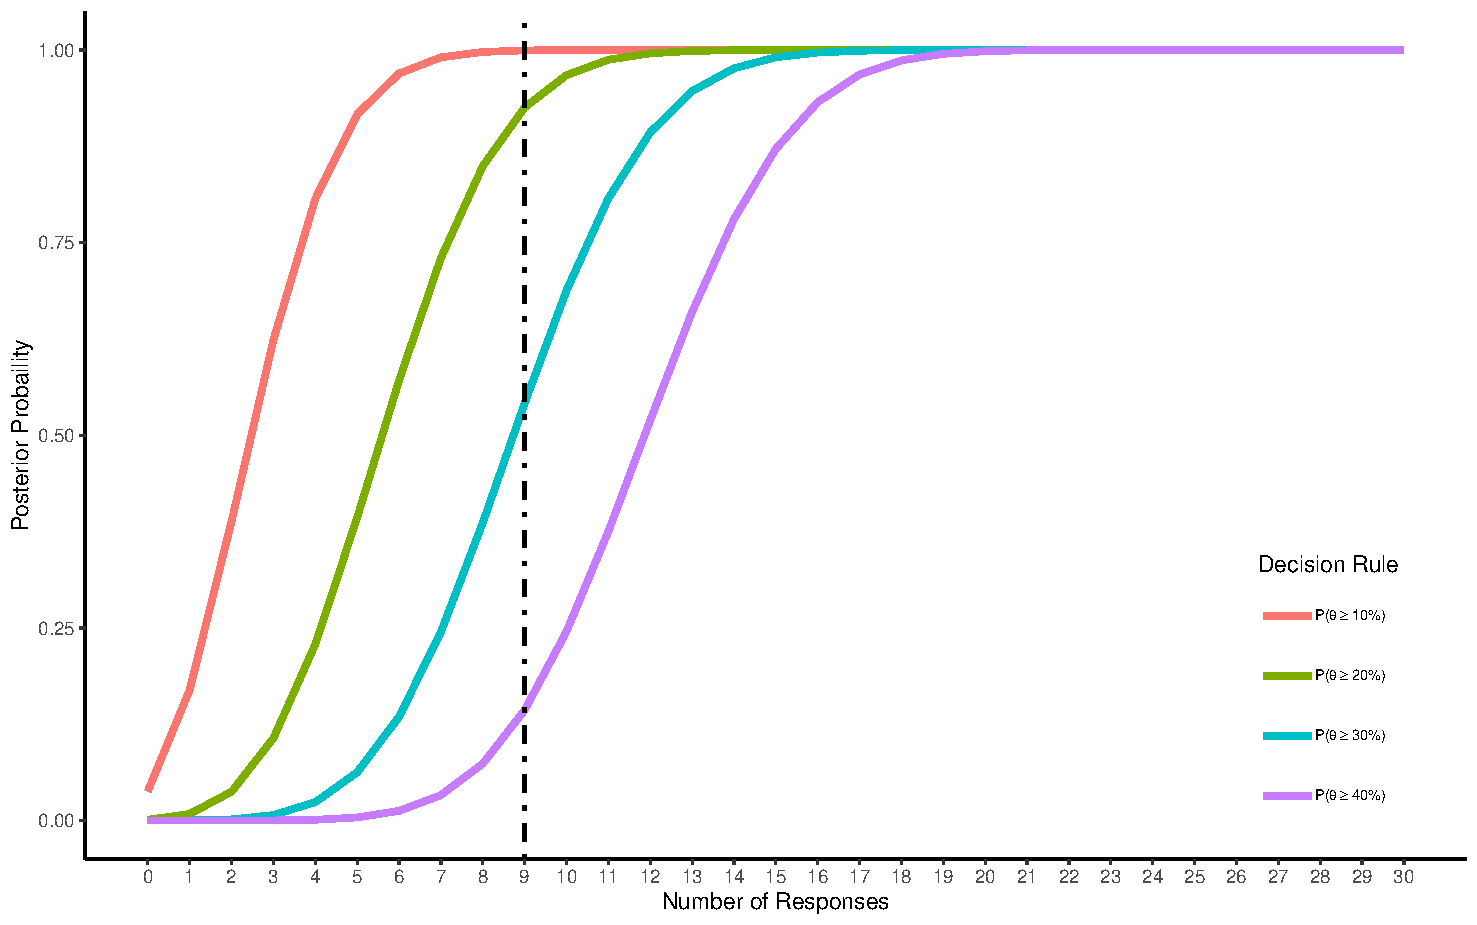
\includegraphics[width=\textwidth]{ETP-DecisionCriteria}
\end{figure}

Here we have shown how ETPs are constructed and how they change and react to modifications in our decision rules. There are several other factors which can impact an ETP such as the prior used in the Beta-Binomial conjugate analysis as well as the timing of each interim analysis and the overall sample size of the trial. Changes to the prior will have an impact on all of the calculations as it is used to generate the posterior distribution on which all of the other calculations are based upon. Adding more interim analyses would add more rows to the plot and changing the sample size of the trial alters the number of cells in each row. 

Overall ETPs can be a useful tool during the design stages of a trial as we can experiment with different decision rules and see what practical affect it has on the trial in terms of the number of responses that need to be observed for a GO decision. They can be used to facilitate discussions with non statistical experts involved in the design of the trial. Much like dose transition pathways in a dose-finding trial they can also provide some transparency as to what decisions will be made and when they would be made. 

A single ETP also provides us with the ability to see how multiple different decision rules may change the outcome for a trial. If just the acceptable probability levels for the PPoS and final analysis, $t$ and $q$, are changing in the decision rule the impact of those changes should be apparent just by comparing the PPoS and posterior probability without the need of generating a whole new plot like we have in our example.

Whilst the calculations needed to produce these plots can be quite simple actually constructing the plots is not so trivial. To overcome this issue and make ETPs easily accessible and producible, we developed a web based application to generate ETPs. All the ETPs shown so far were generated using this application. 

In the next sections we detail trials that have been designed using ETPs. These served as further motivation for development of the application to produce ETPs. We then go on to detail how the app was developed and how it works.    

%----------------------------------------------------------------------------------------
%	SECTION 4
%----------------------------------------------------------------------------------------

\section{Implementation of Efficacy Transition Pathways}

With the development of any new methodology or novel tool such as ETPs there will be some barriers that will impede its use. One of those barriers will be the difficulty of implementing the methodology. If the intention of some newly developed methodology is for it be applied in a practical setting, when presented it should be accompanied by appropriate software or code such that the target audience are able to implement it with minimal effort. Otherwise the new methodology may remain purely theoretical and would rely on others to come up with a solution for its implementation. 

To overcome this barrier for ETPs we developed a R function to produce these plots given the input of key details such as the decision criteria, sample size and cohort size. We then used this function and built a web application around it. Rather than just offering code to implement ETPs a web app makes implementation even easier as it doesn't require knowledge or experience with a specific piece of stats software such as R, STATA or SAS. 

Another barrier that limits the rate at which new methodology is implemented is a lack of awareness or familiarity with the methodology. Specifically, with clinical trials that often involve a multidisciplinary team it is unrealistic to expect clinicians or trial management to be up to date with the latest statistical innovations. Even the statisticians themselves may not be familiar with the latest methodology. As a result, newer methods may be overlooked even if it would be beneficial to implement. Even if statisticians are aware of new methodology, the struggle may then become explaining the methodology to non-statisticians and convincing them it will be beneficial to use. 

Inherently ETPs as a tool were created to help better explain the analysis that is done in these phase \RN{2} trials as well as the decisions that are made. They exist more as a tool to help promote the underlying Bayesian methodology. Therefore ETPs may be simple to implement and explain to non-statisticians. Instead the issue may come from a lack of understanding of a Beta-Binomial conjugate analysis, predictive probabilities or the background methodology behind the ETPs. 

To address this within our web application we included detailed information about ETPs as well as a breakdown of the methodology behind them. This was done through text and images in combination with custom built interactive tools that illustrates how these trials are run in a practical setting. These additional explanations and features were built in to make understanding ETPs easier, especially for those with a non stats background. These sections can also be used as a teaching tool to help educate those who are working on trials but not familiar with this methodology.  

Lucinda Billingham (LB) as the visionary behind ETPs had began implementing them in a number of different trial designs despite these barriers. Some of these trials were being designed as umbrella, basket or platform trials and involved multiple arms. Here analyses and decisions were being made in each arm independently so ETPs were employed to help design these trials. 

This leads to more issues where during the design stages of a trial multiple ETPs may need to be generated. If changes were made to specific decision criteria the ETP would need to be updated so you could communicate how those changes would affect the outcome of the trial. This is then further compounded with the complex trial designs where there may different criteria dependent on the arms in the trial.

Prior to the development of the app ETPs were being constructed by hand which was a time consuming endeavour. We will detail three trials that were designed by the Cancer Research Clinical Trials Unit (CRCTU) at the University of Birmingham and show how ETPs have previously been implemented. 

%-----------------------------------
%	SUBSECTION 1
%-----------------------------------

\subsection{MonoGerm} 

This trial was designed by Lucinda Billingham (LB) and Laura Kirton (LK). What is presented here is the design that was used as part of a grant application which has since been accepted. The trial is currently in the process of being set-up so may be subject to some design changes before it is open. 

MonoGerm \footnote{A phase II trial of carboplatin or vinblastine monotherapy induction prior to radiotherapy for patients with intracranial germinoma} is a Phase \RN{2} trial investigating, in parallel, two single-agent chemotherapies (carboplatin or vinblastine) as monotherapy prior to standard of care radiotherapy in patients with intracranial germinoma. This trial utilises a Bayesian approach for analysis and decision making. A 'flip-flop' approach is used for recruitment \cite{harringtonGuidelinesPreclinicalEarly2011}. Essentially, recruitment will begin to the carboplatin arm then once three patients have been recruited and considered evaluable for an interim analysis recruitment flips to the vinblastine arm. This process is then repeated by switching recruitment back and forth between the two arms till recruitment is complete. 

Typically intracranial germinoma is chemosensitive but it requires radiotherapy for a cure. This mainly affects a paediatric population. For patients with localised disease standard of care involves three-drug chemotherapy consisting of ifosfamide, carboplatin and etoposide followed by subsequent radiotherapy. Treatment involving multiple chemotherapies allows for reduction in radiotherapy doses and fields. However, there is still an increased burden of treatment on patients which can cause both short and long-term harm. This can lead to patients experiencing multiple toxicities such as diabetes insipidus, myelosuppression, vomiting/diarrhoea, electrolyte disturbances, renal impairment, and elevation of liver enzymes. 

The aim of the trial is to evaluate whether a single-agent chemotherapy (carboplatin or vinblastine) is non-inferior to	the standard of care multi-drug chemotherapy for inducing complete response (CR), and is associated with reduced harm and improved quality of life. The primary outcome measure will be CR based on MRI scans at 6 and 12 weeks. 

The trial will consist of two arms, one arm for carboplatin and one for vinblastine. There will be 36 patients recruited in total, 18 per arm. Patients will be enrolled in cohorts of three to each treatment-arm by the flip-flop design. This is illustrated in Figure \ref{fig_etp:MonoGermFlipFlop}. Recruitment begins in the carboplatin arm and then once three patients have been recruited recruitment is paused and then begins in the vinblastine arm. Whilst recruitment is paused in the carboplatin arm an interim analysis will be performed for that first cohort. Here primary outcome data and key safety data will be assessed. Once recruitment to the first cohort of the vinblastine arm is complete and the interim analysis for the first cohort of carboplatin patients is done recruitment can begin for the second cohort in the carboplatin arm and the interim analysis for the first cohort of vinblastine patients can be conducted. This process is then repeated for the subsequent cohorts. This design allows for continuous enrolment and monitoring of the primary outcome. 

\begin{figure}[h!]
	\centering
	\caption{Flip-flop recruitment design in the MonoGerm trial.}
	\label{fig_etp:MonoGermFlipFlop}
	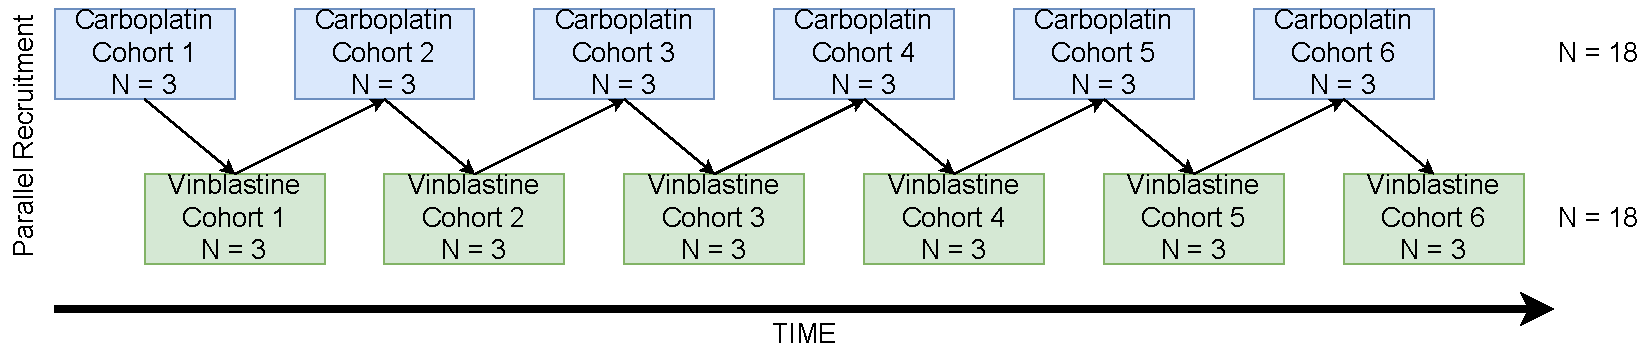
\includegraphics[width=\textwidth]{ETP-MonoGermFlipFlop}
\end{figure}

A Bayesian approach is implemented to assess the true CR rates. Specifically, the experimental monotherapies will need to demonstrate non-inferiority to the standard of care by a clinically acceptable margin. Based on previous data it was determined that the minimum CR rate with standard of care is 30\%. This value was taken as the non-inferiority margin. So, if the treatments have a CR rate $\geq30$\% they will be considered non-inferior. 

CR rates for each treatment arm will be established from the posterior probability distribution generated using a beta-binomial conjugate analysis. A minimally informative Beta(1,1) prior will be used in combination with the data observed during the trial to produce the posterior. In terms of decision making the following rule for the final analysis was specified: 

\begin{equation}
	P(CR \geq 30) \geq 0.8
\end{equation}

That is to say that if there is a high probability ($\geq 0.8$) that the true CR rate is $\geq30$\% there will be a GO decision. Which in the context of this trial means the treatment arm would be deemed non-inferior. The minimum number of observed CRs out of the 18 patients needed to warrant a GO decision is seven. If seven responses are observed the median Bayesian estimate of the CR rate would be 40\% with a 0.82 probability that the true CR rate is $\geq30$\%. 

Stopping rules have also been implemented. At each interim analysis the predicted probability of success (PPoS) will be calculated. This is the probability that a GO decision would be made at the final analysis based on current data that has been accrued. Here the stopping rule is such that if the PPoS is less than 0.01 we would recommend stopping recruitment to that arm. 

It is important to note that whilst the trial has two arms it is not designed with the intention of making comparisons between the two treatments. Rather the trial aims to find if there is enough evidence that one of these treatments provides a sufficient response rate to warrant a GO decision.  

LK produced ETPs throughout the design of this trial. Figure \ref{fig_etp:MonoGermETP} shows the ETP for the design specified here. The ETPs produced here helped determine what data we wanted to present as well as how we structure the data in each of the cells. Here each cell shows the number of responses, the PPoS or the posterior probability that the response rate is $\geq30$\%, the Bayesian estimate of CR rate and a lower one-sided 80\% credible interval.

Calculations for these plots were conducted in STATA and the ETP was produced in Microsoft PowerPoint. One benefit of this approach is that the ETP can be easily customised and labelled. However, this meant that any changes in the design that affected the decision-making resulted in the ETP having to be updated manually. As a tool the ETP is effective at illustrating a final design but without the ability to easily generate them during the design of a trial they somewhat lose their purpose. This served as further motivation to produce some code or a tool that would allow for ETPs to be automatically created. 

\begin{sidewaysfigure}[h!]
	\centering
	\caption{ETP for the MonoGerm trial.}
	\label{fig_etp:MonoGermETP}
	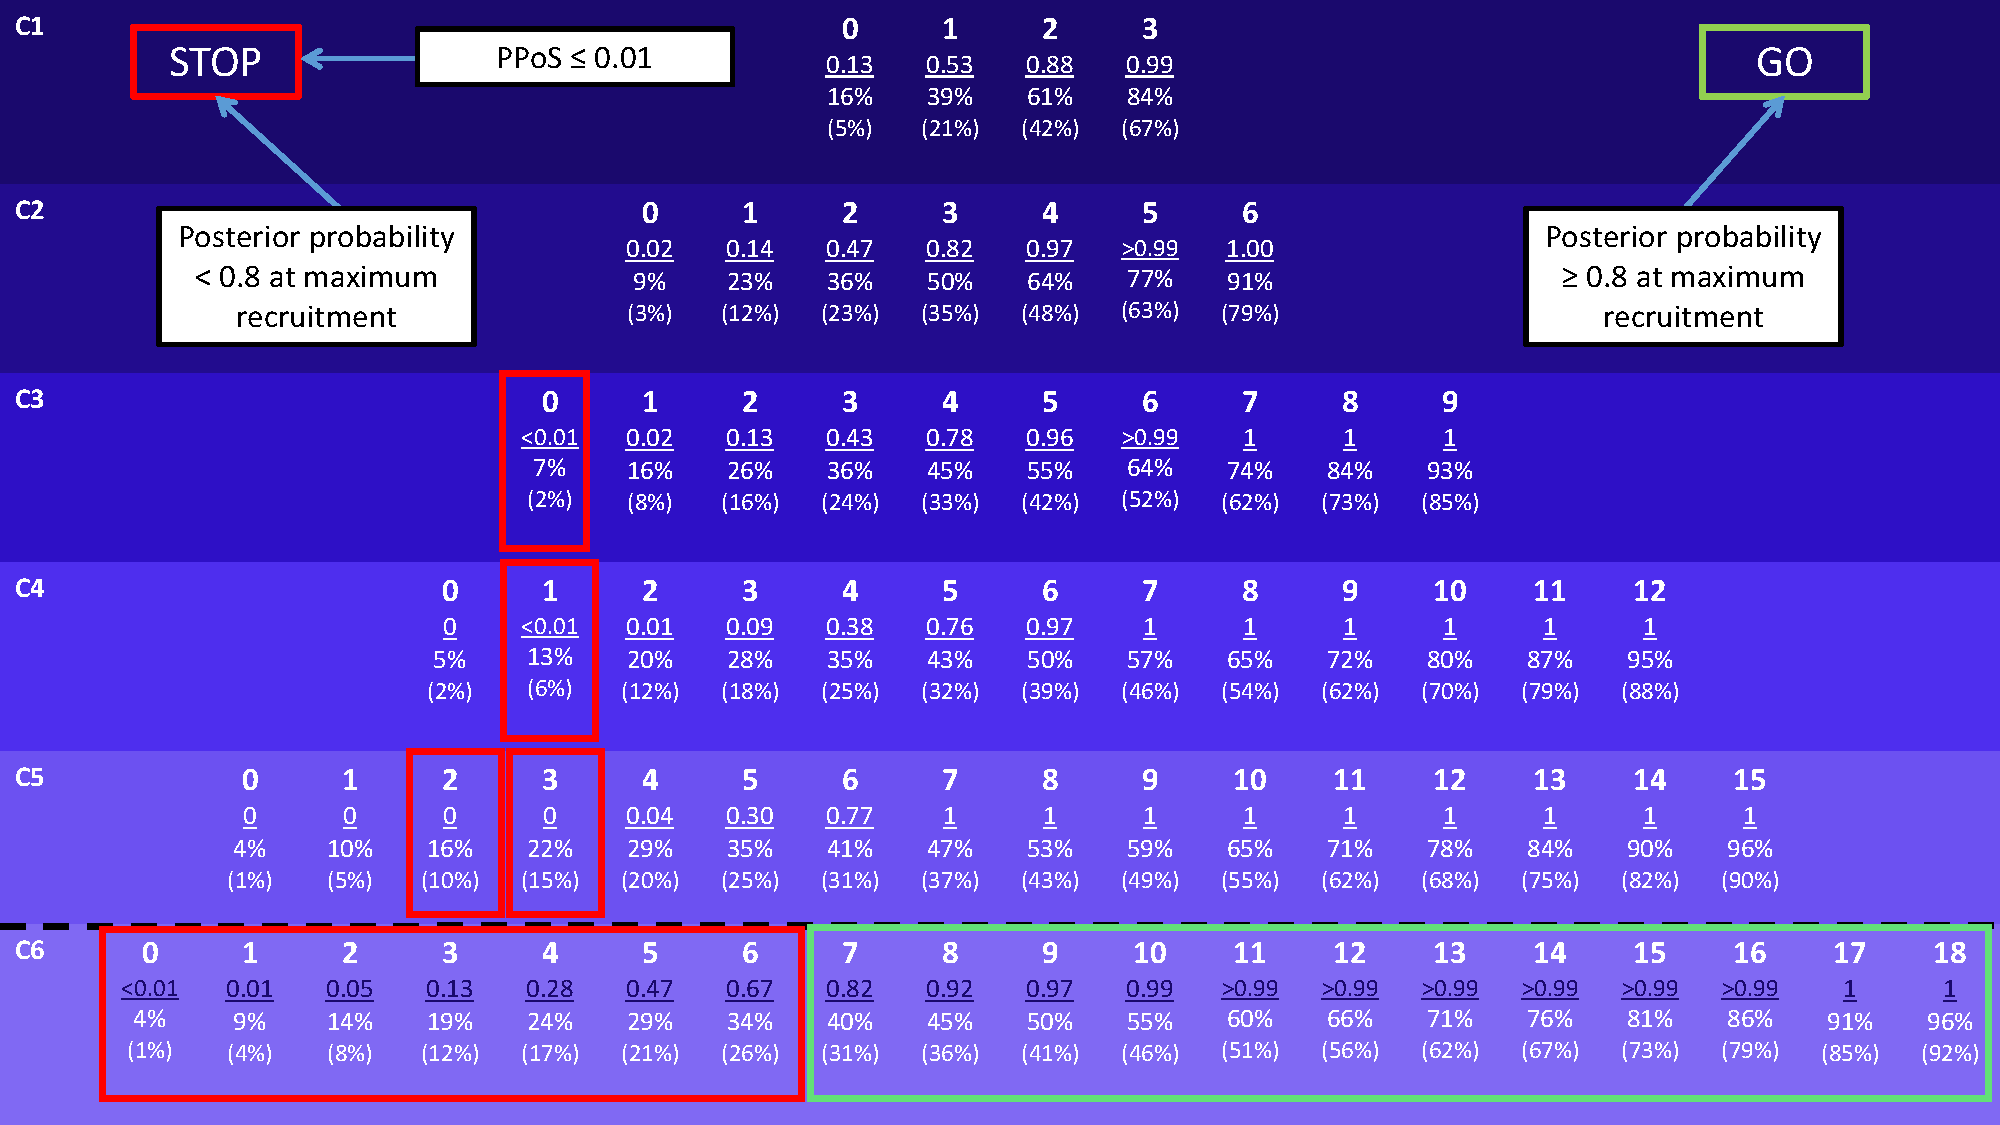
\includegraphics[width=23cm, height=15cm]{ETP-MonoGermETP}
\end{sidewaysfigure} 

\clearpage

%-----------------------------------
%	SUBSECTION 2
%-----------------------------------

\subsection{Glo-BNHL}

This trial was designed by Lucinda Billingham (LB) with the assistance of Shanna Maycock (SM). During initial stages of the design Grace Holt (GH) also assisted with the implementation of ETPs. This trial is currently still in set-up so specific details of the trial may be subject to change.   

The Glo-BNHL \footnote{A Global Study of Novel Agents in Paediatric and Adolescent Relapsed and Refractory B-cell Non-Hodgkin Lymphoma} study is a platform trial that aims to investigate the safety and effectiveness of novel treatments in children, adolescents and young adults with relapsed and/or refractory B-cell non-Hodgkin Lymphoma (r/r BNHL). This trial is an international collaboration and hopes to generate substantial evidence that could change practice in this rare cancer population. 

Inclusion of novel agents into the platform will be determined by an international Trial Steering Committee (TSC). Currently the platform consists of three separate treatment arms, each focusing on a different novel agent in a distinct group of patients. Each treatment arm will be treated independently which allows for them to be analysed separately. There may also be separate eligibility criteria for each arm. Patients will be enrolled into any arm where they are eligible. The three arms that will be available at the start of the trial are as follows: 

\begin{itemize}
	\item Treatment Arm \RN{1}: Bispecific Antibody (BsAb)
	\item Treatment Arm \RN{2}: Antibody-Drug Conjugate (ADC) with standard \\ chemotherapy
	\item Treatment Arm \RN{3}: Chimeric Antigen Receptor (CAR) T-cells
\end{itemize}

This trial utilises an adaptive Bayesian design, which enables GO/No GO decisions specific to the distinct populations in each treatment arm. The Bayesian approach has many benefits here as it facilitates decision making with small sample sizes. Decisions will be made based on the estimate of the probability that a novel agent is clinically effective. The specific criteria will vary between each treatment arm. This design and approach also allows for continuous evaluation of each novel agent. Treatment arms may be removed if the treatment is shown to be ineffective based on the trial data. Additionally, treatment arms may also be added or amended in the future if recommended by the TSC. 

Treatment arm \RN{1} aims to estimate the clinical efficacy of BsAb treatment in patients with r/r BNHL in first (only one prior line of therapy) or subsequent relapse (more than one prior line of therapy). Due to this treatment arm \RN{1} is split into two groups, \RN{1}a and \RN{1}b for patients with one relapse or more than one relapse respectively. These two subsequent arms will be recruited into and analysed separately. In terms of treatment these patients will receive odronextamab given as an intravenous infusion weekly for 12 weeks, then every two weeks until nine months, and every four weeks thereafter until progression or for a maximum of two years. The outcome measure for patients in treatment arms \RN{1}a and \RN{1}b is the occurrence of an objective response (OR) i.e. complete response (CR) or partial response (PR) after 12 weeks of treatment assessed by Independent Central Review. However, for interim analyses local response assessments will be used. 

Treatment arm \RN{2} aims to estimate the clinical efficacy of ADC treatment with modified R-ICE (rituximab, ifosphamide, carboplatin, etoposide and dexamethasone) chemotherapy in patients with r/r B-NHL in first or subsequent relapse. Patients will receive loncastuximab tesirine given as a 30 minute intravenous infusion with each cycle of modified R-ICE for a maximum of three cycles. Here the outcome measure is occurrence of CR within a maximum of three cycles of treatment. 

Treatment arm \RN{3} aims to estimate the efficacy of CAR T-cell therapy in r/r B-NHL patients who have CAR T-cell product available. The specific treatments patients will receive is yet to be defined. The outcome measure is the occurrence of OR following CAR T-cell infusion. 

Each treatment arm and subsequent treatment arm (i.e. \RN{1}a and \RN{1}b) will aim to recruit 15 evaluable patients during the initial stage. Once this recruitment is complete a transition analysis is performed leading to three possible outcomes. If the analysis results in a No GO decision recruitment to that treatment arm will stop. If the analysis result is a GO decision there are two options either there is sufficient evidence to change practice so the trial will stop recruiting or this will trigger an expansion stage in which a further 15 patients will be recruited. Following the expansion stage a confirmatory analysis will be conducted on all 30 evaluable patients. 

Interim analyses will be conducted after every three patients during the initial stage and after every five patients during the expansion stage. There will also be the option to stop recruitment to a treatment arm based on the data observed in the interim analysis. Figure \ref{fig_etp:Glo-BNHLflowchart} shows a flowchart of the decision making process for each arm in the trial. 

\begin{figure}[h!]
	\centering
	\caption{Flowchart of the decision making process in Glo-BNHL.}
	\label{fig_etp:Glo-BNHLflowchart}
	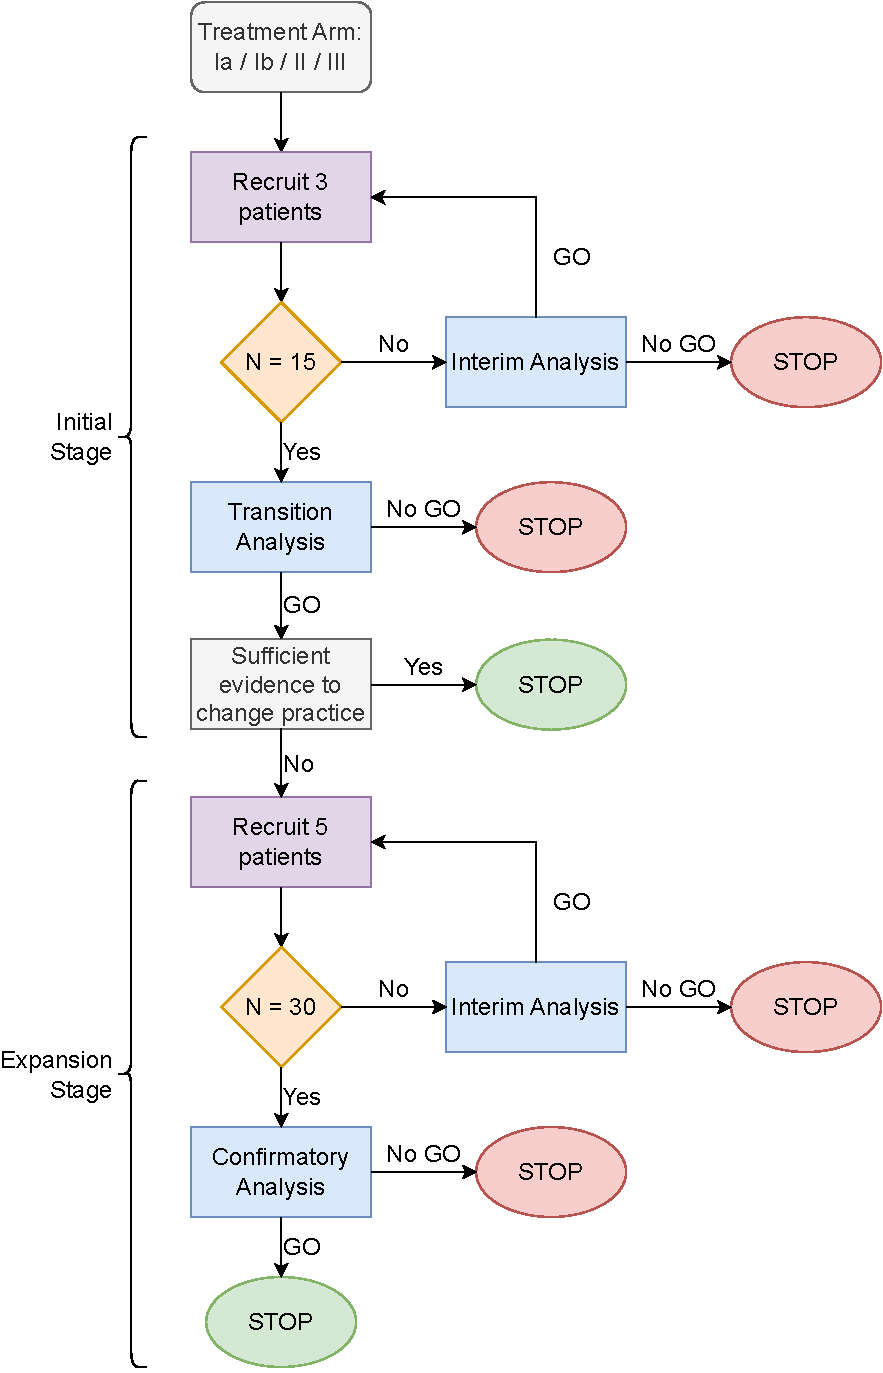
\includegraphics[width=0.9\textwidth]{ETP-GloBNHL-flowchart}
\end{figure}

A beta-binomial conjugate analysis will be conducted for each treatment arm. Observed trial data will be combined with a minimally informative Beta(1,1) prior to produce a posterior probability distribution for the treatment effect $\theta$, which represents either the OR/CR rate dependent on treatment arm. The posterior probability distribution is then used to inform decision making. GO/No Go decision criteria are specified separately for each treatment arm. 

For treatment arm \RN{1}a the decision criteria at the transition analysis is P($\theta$ > 40\%) $\geq$ 0.8. So, if the true OR rate was greater than 40\% with a probability of at least 0.8 based on the data collected in the trial there would be a GO decision. This corresponds to observing at least eight responses out of 15. For the confirmatory analysis a GO decision is made if P($\theta$ > 40\%) $\geq$ 0.95. At the final analysis we would need the probability that the true OR rate was greater than 40\% to be at least 0.95. Here a GO decision would only be made if 17 out of 30 patients had an OR. Table \ref{tab_etp:GloBNHL_decision_criteria} details the criteria for each treatment arm which can be interpreted in a similar manner. 

\begin{table}[h!]
	\centering
	\caption{Summary of decision criteria for Glo-BNHL.}
	\label{tab_etp:GloBNHL_decision_criteria}
	\resizebox{\textwidth}{!}{%
		\begin{tabular}{ccccc}
			\hline
			\multicolumn{1}{l}{\textbf{}} & \multicolumn{2}{c}{\textbf{Transition Analysis}}               & \multicolumn{2}{c}{\textbf{Confirmatory Analysis}}             \\ \cline{2-5} 
			\textbf{Treatment Arm}        & \textbf{Decision Criteria} & \textbf{Min No. Responses for GO} & \textbf{Decision Criteria} & \textbf{Min No. Responses for GO} \\ \hline
			Ia  & P($\theta$ \textgreater 40\%) $\geq$ 0.8 & 8/15 & P($\theta$ \textgreater 40\%) $\geq$ 0.95 & 17/30 \\
			Ib  & P($\theta$ \textgreater 10\%) $\geq$ 0.8 & 3/15 & P($\theta$ \textgreater 10\%) $\geq$ 0.95 & 6/30  \\
			II  & P($\theta$ \textgreater 20\%) $\geq$ 0.8 & 5/15 & P($\theta$ \textgreater 20\%) $\geq$ 0.95 & 10/30 \\
			III & P($\theta$ \textgreater 10\%) $\geq$ 0.8 & 3/15 & P($\theta$ \textgreater 10\%) $\geq$ 0.95 & 6/30  \\ \hline
		\end{tabular}%
	}
\end{table}

For the interim analyses there are separate stopping rules. These are the same across the treatment arms but differ in the initial stage compared to the expansion stage. During the initial stage, the predicted probability of success at the transition analysis (PPoSt) is calculated and decisions are made based on the following criteria: 

\begin{enumerate}
	\item PPoSt < 0.01 - recommend stopping for futility
	\item 0.01 $\leq$ PPoSt < 0.05 - consider stopping for futility
	\item 0.05 $\leq$ PPoSt < 0.15 - consider whether sufficient benefit in continuing 
	\item PPoSt $\geq$ 0.15 - recommend continuing 
\end{enumerate}

So, if the probability of success at the transition analysis is less than 1\% the recommendation would be to stop recruitment to the treatment arm and if it was greater than or equal to 15\% the recommendation would be to continue recruitment. If PPoSt is between 1-5\% or 5-15\% stopping should be also be considered for either futility or if there sufficient benefit in continuing respectively.  

At the expansion stage, the predicted probability of success at the confirmatory analysis is used (PPoSc). If this is below 10\% (PPoSc < 0.1) the recommendation would be to stop recruitment to that treatment arm due to futility. It should be noted that these decision rules are only recommendations and the independent data monitoring committee (DMC) will make decisions based on not only primary outcomes but secondary outcomes, recruitment and safety data. 

For this trial ETPs were produced separately for each treatment arm and for each stage. This resulted in eight ETPs, one for the initial stage showing the outcome of the transition analysis and one for the expansion stage showing the outcome of the confirmatory analysis for each treatment arm (\RN{1}a, \RN{1}b, \RN{2}, \RN{3}). ETPs were utilised throughout the design of the trial with initial versions originally created by GH using STATA and Microsoft PowerPoint. These were then further developed by SM who performed calculations in R but still utilised PowerPoint to create the ETPs. Figure \ref{fig_etp:GloBNHL-ETP-TA1aInitial} and \ref{fig_etp:GloBNHL-ETP-TA1aExtenstion} shows the ETPs for the initial and expansion stage of treatment arm \RN{1}a respectively. These ETPs created by SM helped us determine how our function and app visually presented ETPs and we utilised a similar colour scheme. 

Similar to MonoGerm the process of creating these ETPs in PowerPoint can be time consuming. This is even more of an issue in the Glo-BNHL study due to the multiple treatment arms and stages. Additionally, this trial highlighted another issue when you have multiple statisticians working on a trial who use different software packages. In this case it would mean work would have to be recreated in R and STATA to conduct the calculations required for ETPs. This served as further motivation for the development of an application which requires no specific stats software knowledge. As statisticians would easily be able to recreate ETPs. SM went on to further extend the function we developed to automatically generate ETPs specific to Glo-BNHL. 

\begin{sidewaysfigure}[h!]
	\centering
	\caption{ETP for the initial stage of treatment arm \RN{1}a in Glo-BNHL.}
	\label{fig_etp:GloBNHL-ETP-TA1aInitial}
	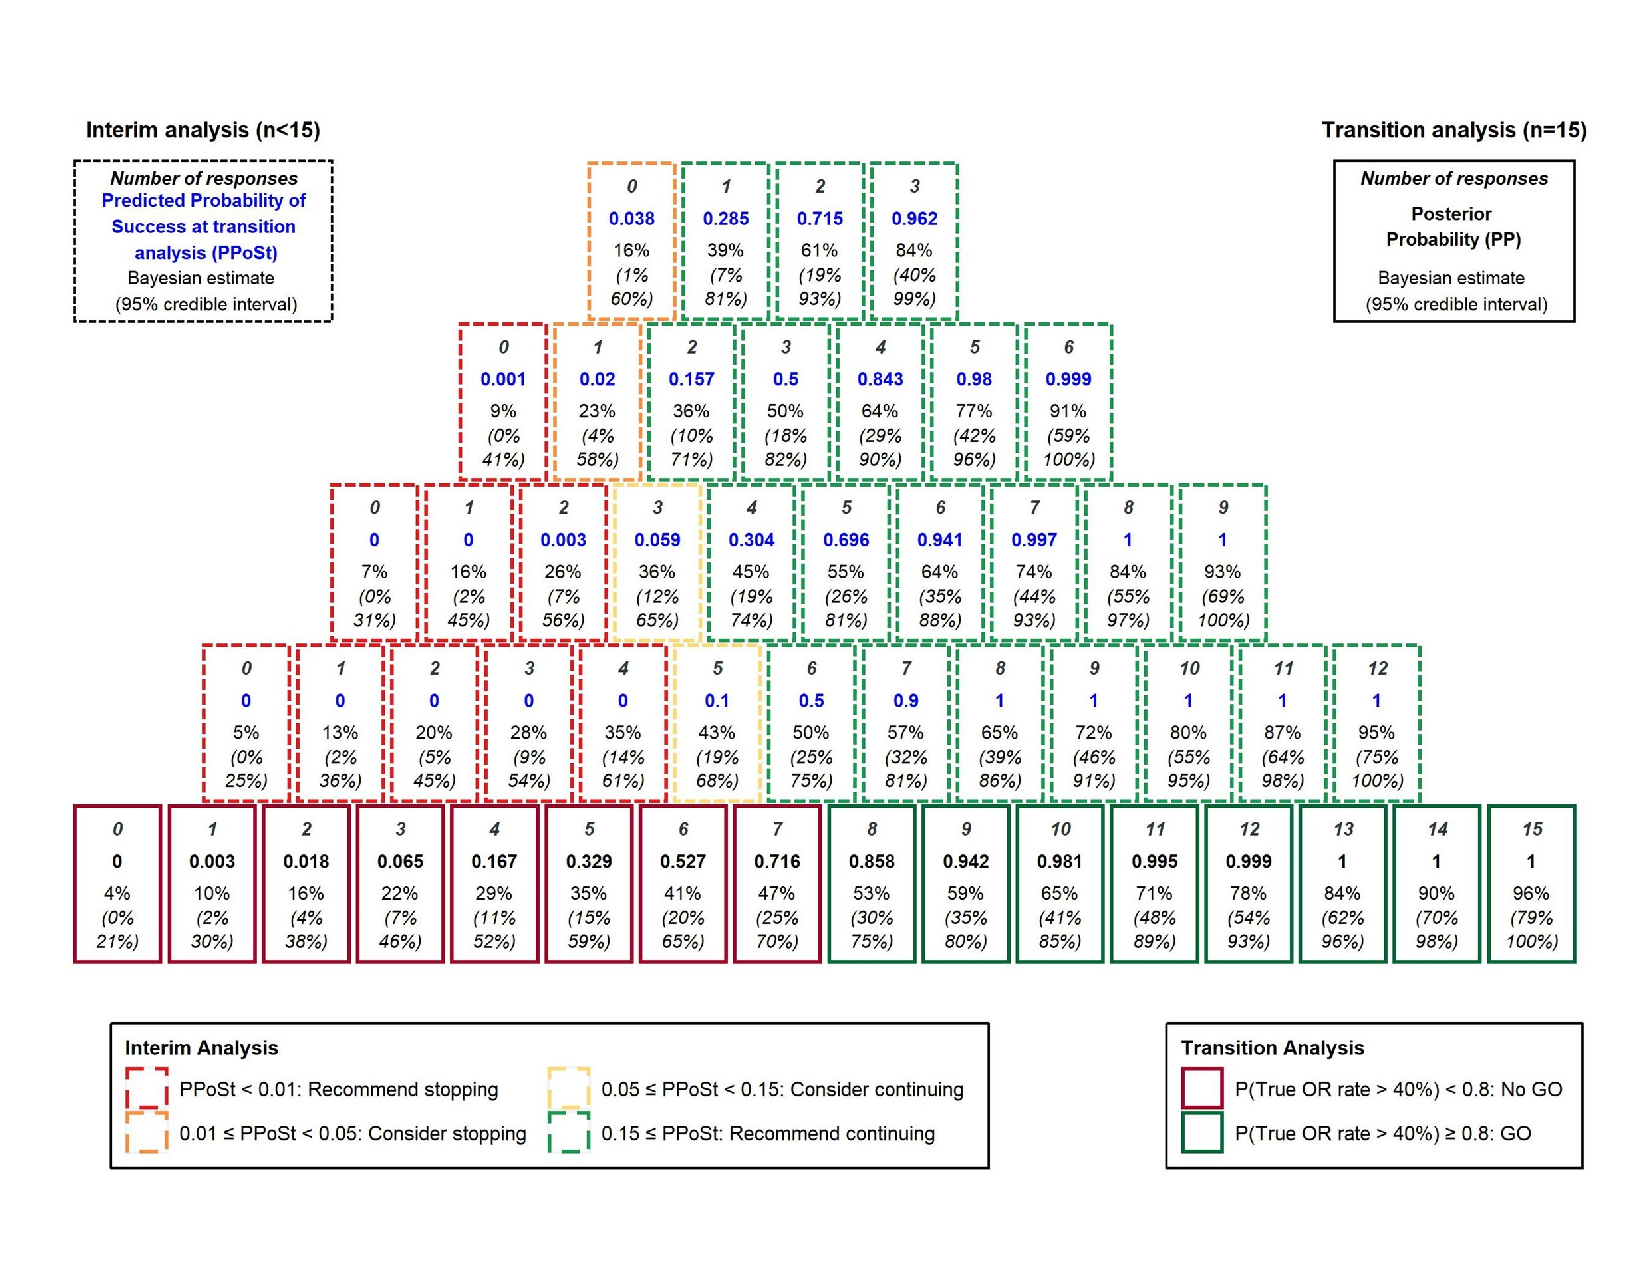
\includegraphics[width=23cm, height=15cm]{ETP-GloBNHL-ETP-TA1aInitial}
\end{sidewaysfigure} 

\begin{sidewaysfigure}[h!]
	\centering
	\caption{ETP for the expansion stage of treatment arm \RN{1}a in Glo-BNHL.}
	\label{fig_etp:GloBNHL-ETP-TA1aExtenstion}
	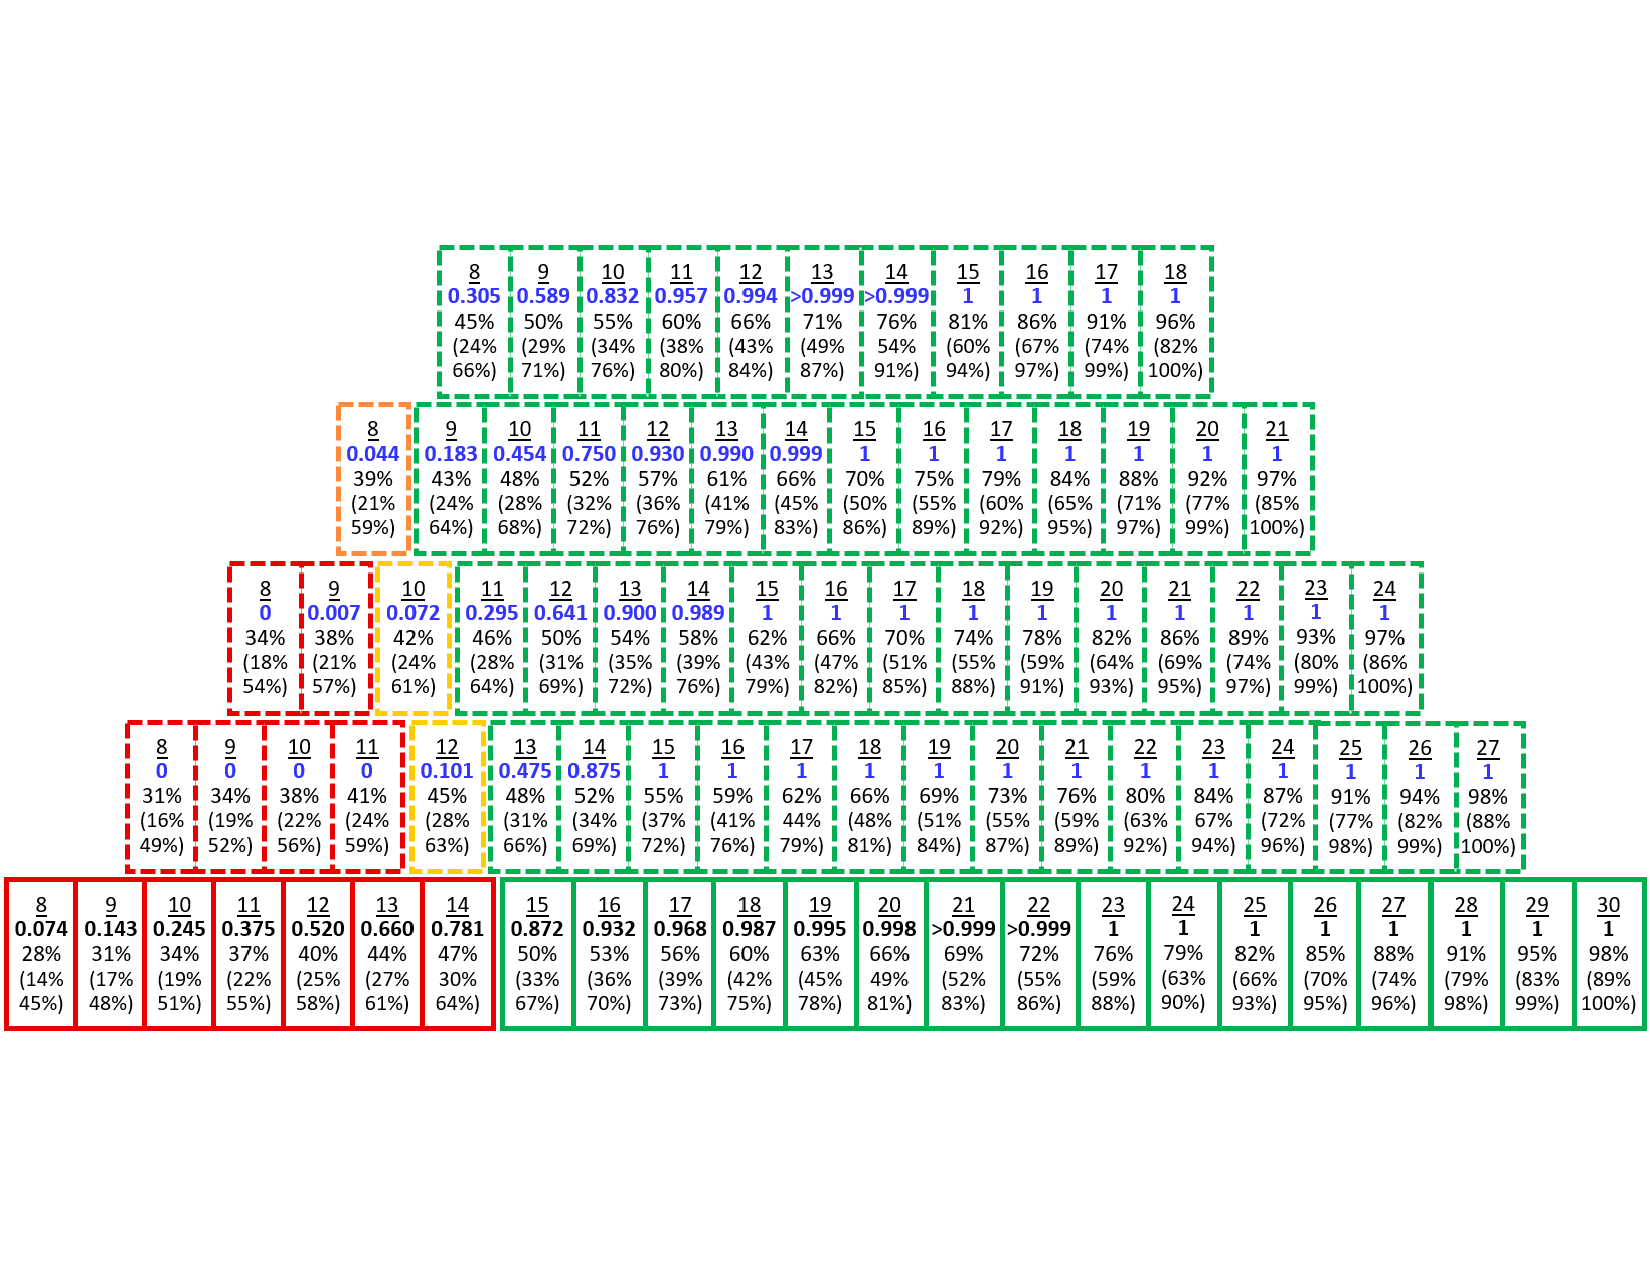
\includegraphics[width=23cm, height=15cm]{ETP-GloBNHL-ETP-TA1aExtension}
\end{sidewaysfigure} 

\clearpage

%-----------------------------------
%	SUBSECTION 3
%-----------------------------------

\subsection{DETERMINE}

DETERMINE \footnote{Determining Extended Therapeutic indications for Existing drugs in Rare Molecularly-defined Indications using a National Evaluation platform trial} is a trial that was also designed by Lucinda Billingham (LB). It is an umbrella-basket platform trial with multiple treatment arms running in parallel. The trial aims to evaluate the efficacy of targeted therapies in rare cancers with actionable genomic alterations, including common cancers with rare actionable alterations. This trial is currently open to recruitment and may be expanded in the future as more drugs are bought onto the platform.  

DETERMINE will recruit patients of all ages including, paediatric, TYA (teenage and young adult) and adults, who have rare tumours that contain an actionable genetic alteration that can be targeted therapeutically. The genetic alteration must have been identified previously from a tissue biopsy or ctDNA (circulating tumour DNA). Patients will then be stratified into molecular groups based on their tumour profile and allocated to the most suitable treatment arm by the Molecular Tumour Board (MTB). The umbrella part of the design consists of multiple non-randomised treatment arms, each evaluation a licensed targeted anti-cancer drug or drug combination in a specific molecularly-defined group of patients. Each molecularly-defined group allocated to a specific treatment arm will contain multiple baskets of different tumour types, age groups and molecular subtypes. This is visualised in Figure \ref{fig_etp:DETERMINEDesign}. 

\begin{figure}[h!]
	\centering
	\caption{Umbrella-basket platform trial design in DETERMINE.}
	\label{fig_etp:DETERMINEDesign}
	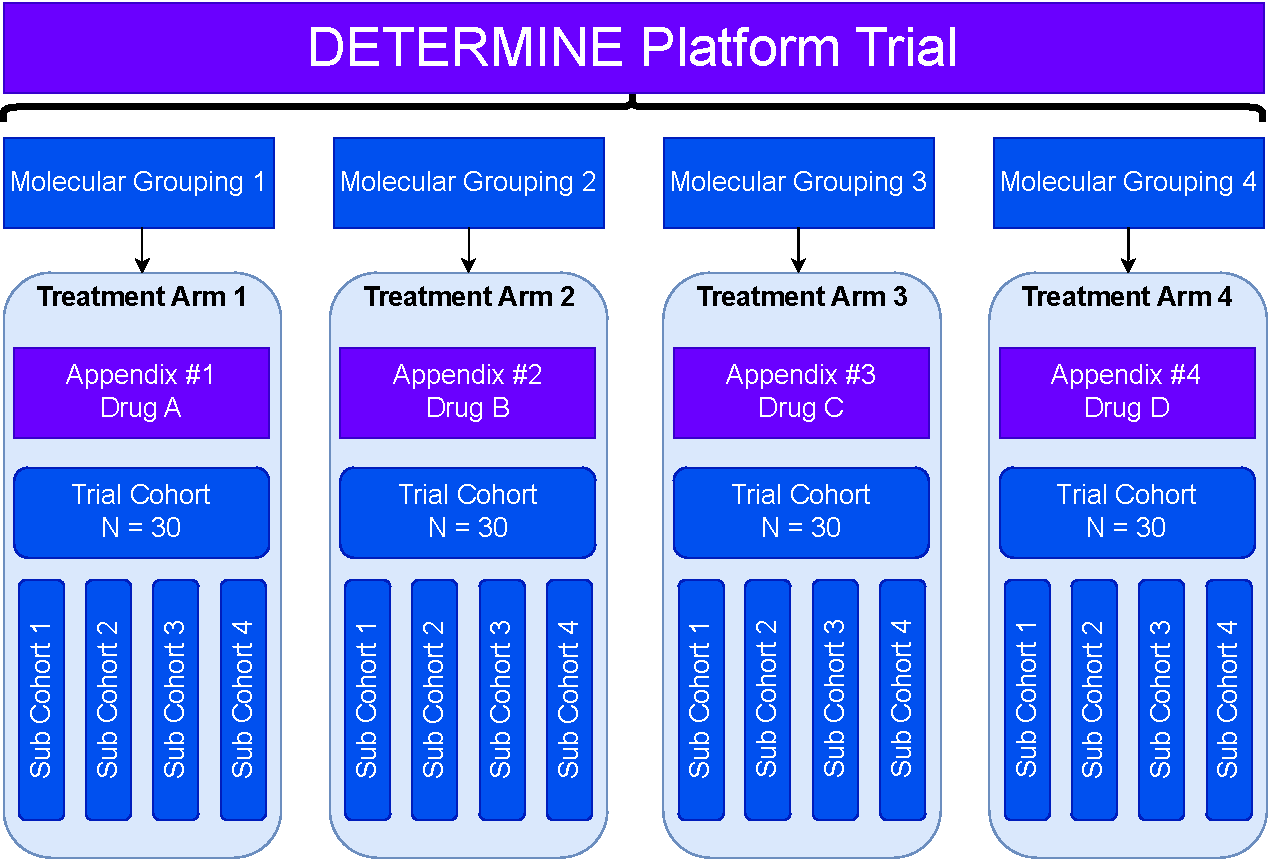
\includegraphics[width=\textwidth]{ETP-DETERMINEDesign}
\end{figure}

A main trial cohort of 30 evaluable patients will be recruited into each treatment arm. This will include patients with different tumour types, ages and molecular subtypes. If specific subgroups within this main cohort are experiencing significant benefit from treatment sub-cohorts will be formed to investigate treatment effectiveness in these subgroups. It is possible for each treatment arm to have multiple sub-cohorts and they can recruit in parallel to the main cohort. Each sub-cohort will be subject to the same statistical analysis and will also aim to recruit 30 patients. Currently there are five treatment arms, details of these are provided in Table \ref{tab_etp:DETERMINE_trtarms}. 

\begin{table}[h!]
	\fontsize{10pt}{10pt}\selectfont
	\centering
	\caption{Current treatment arms in DETERMINE}
	\label{tab_etp:DETERMINE_trtarms}
	\resizebox{\textwidth}{!}{%
		\begin{tabular}{p{0.1\textwidth} | p{0.2\textwidth} | p{0.5\textwidth} | p{0.2\textwidth}}
			Treatment Arm  & IMP(s) & Molecular Grouping & Route and Formulation \\ \hline
			1 &  Alectinib & ALK gene fusion positive solid tumours & Oral capsules \\ \hline
			2 & Atezolizumab & Solid tumours with high tumour mutational burden (TMB) or microsatellite instability-high (MSI-high) or proven constitutional mismatch repair deficiency (CMMRD) disposition & Intravenous (IV) infusion  \\ \hline
			3 & Entrectinib & NTRK or ROS1 gene fusion positive solid tumours & Oral capsules; Dosing depends on body surface area (BSA) \\ \hline
			4 & Trastuzumab in combination with pertuzumab & Solid tumours with HER2 amplification or mutations & IV infusion \\ \hline 
			5 & Vemurafenib in combination with cobimetinib & Solid tumours with BRAF V600 mutations & Oral; 960 mg tablets \\ \hline
		\end{tabular}
	}
\end{table}

Co-primary outcomes of objective response (OR) and durable clinical benefit (DCB) will be used to assess efficacy of the treatment in each of the cohorts in each molecular grouping. These are both classified as binary variables. OR is defined dependent on specific disease criteria. DCB is defined as the absence of disease progression for at least 24 weeks from the start of trial treatment, this will also be measured based on disease specific criteria. Patients will receive treatment based on the license schedule for the drug in their treatment arm. Patients continue treatment until either they reach progressive disease (PD), unacceptable adverse events or withdraw from the trial. 

All outcomes in each treatment arm, cohort and sub cohort will be analysed using a Beta-Binomial conjugate analysis. Posterior probability distributions for OR and DCB will be generated using minimally informative priors, Beta(0.1,0.9) and data that is collected on the trial. However decision making will be done using the BOP-2 design \cite{zhouBOP2BayesianOptimal2017,zhouBayesianOptimalPhase2020}. This design makes GO or No GO decisions by assessing posterior probabilities for a set of outcomes, which are optimised to either maximise power or minimise the number of patients. The design also allows for the control of type I and type II error rates. In DETERMINE, for each co-primary outcome, a rate of 10\% or less would represent a treatment effect that is not clinically relevant and a rate of 30\% would represent a clinically meaningful treatment effect. These can be thought of as a null and alternative hypothesis. The use of this design was made possible due to the development of web applications by the authors at the MD Anderson Cancer Centre \cite{tidwellBayesianClinicalTrials2019}. 

Interim analyses will be conducted throughout the trial, however formal decision making will first be conducted after 10 evaluable patients have been recruited and then every 5 patients from that time-point in each cohort/sub-cohort. If probability that both the true OR and DCB rates are lower than the critical threshold of 10\% the trial would recommend stopping. The design is optimised to minimise the type II error i.e. to minimise the probability of not rejecting the null hypothesis when treatment is effective. This is done whilst controlling the type I error rate at 0.1. Under the BOP-2 design this provides the following stopping boundaries of 0/10, $\leq$1/15, $\leq$2/20, $\leq$3/25 at each of the planned analyses at 10, 15, 20 and 25 patients. For the final analysis at 30 patients there would be a GO decision if $\geq$6/30 patients had either a OR or DCB.   

The ETPs we have shown so far all have been based on a Beta-Binomial conjugate analysis with decisions made using PPoS and the posterior distribution. However, they can also be utilised here. LB created the ETP shown in Figure \ref{fig_etp:DETERMINE-ETP}. Here we can see each cell still pertains to a specific number of responses out of a certain number of patients. Bayesian estimates, credible intervals and posterior probabilities of the treatment effect being greater than our null and alternative hypothesis. The cells have then been colour coded based on the decision criteria elicited from the BOP-2 design. This trial also shows that ETPs are a flexible tool that can also be applied to trials not explicitly using a Beta-Binomial conjugate analysis for decision making. 

\begin{sidewaysfigure}[h!]
	\centering
	\caption{ETP for the DETERMINE trial.}
	\label{fig_etp:DETERMINE-ETP}
	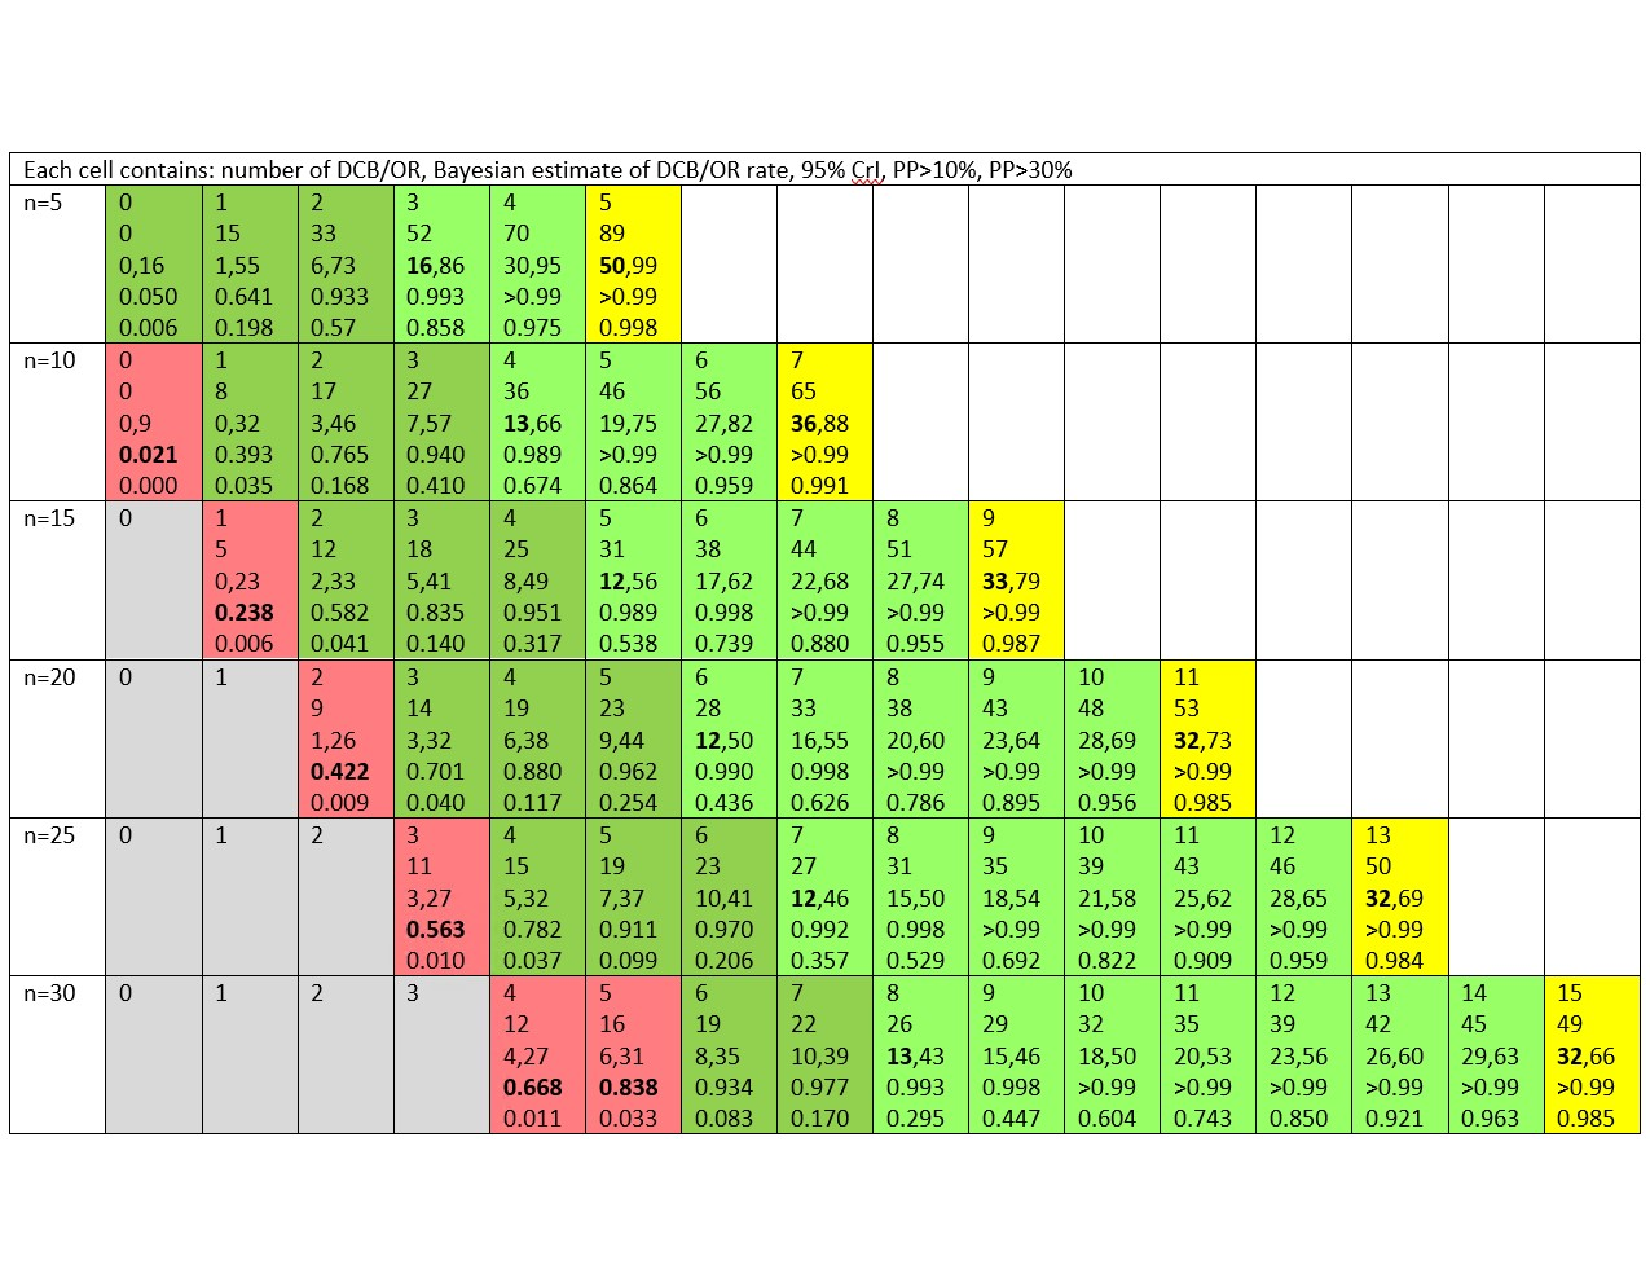
\includegraphics[width=23cm, height=15cm]{ETP-DETERMINE-ETP}
\end{sidewaysfigure} 

\clearpage

%-----------------------------------
%	SECTION 4
%-----------------------------------

\section{Development of a Web Application for Efficacy Transition Pathways}

R shiny \cite{changShinyWebApplication}  is a tool available in R to facilitate the production of interactive web applications (apps). It allows R users to create useful and accessible tools that would otherwise be out of reach of non R users without requiring any programming or statistical knowledge. In the context of medical statistics the usefulness of these types of apps is also acknowledged by funding bodies such as the NIHR (National Institute for Health and Care Research). They have awarded grants which in part helped the development of apps relating to network meta-analysis \cite{owenMetaInsightInteractiveWebbased2019} and meta-analyses of diagnostic test accuracy studies \cite{freemanDevelopmentInteractiveWebbased2019, patelGraphicalEnhancementsSummary2021}. 

Even without funding there have been apps that have been developed to help address issues around the implementation of early phase and adaptive designs. For example, there is a whole suite of software and shiny applications made available by the MD Anderson Cancer Centre \cite{tidwellBayesianClinicalTrials2019} to help implement methodology they have developed. Wheeler et al. \cite{wheelerAplusBWebApplication2016} produced the A plus B app to produce operating characteristics for A+B trial designs \cite{linStatisticalPropertiesTraditional2001}. There is also the MoDEsT app created by Pallmann et al. \cite{pallmannDesigningEvaluatingDoseescalation2020} for designing and conducting single-agent dose-finding trials. Grayling and Wason \cite{graylingWebApplicationDesign2020} developed an app to aid the implementation of multi-arm clinical trial designs. These are just a few examples of shiny apps already available, all of which aim to make certain methodologies more accessible and is something we also wanted to do for ETPs. 

Initially we produced a R function that was able to create ETPs. Then using R shiny an application was built which utilised this function to produce ETPs. Whilst the R function makes implementing ETPs a lot easier, the R shiny app offers an even better solution. Firstly, it doesn't require any previous knowledge of a specific statistical package so any statistician should be able to use the application with ease. This also applies for non-statisticians and an application would make ETPs more accessible.  

R shiny also has the ability to make graphs interactive. Whilst ETPs produce a lot of information they are static in nature. As such a change in parameters or design characteristics means that a separate ETP would need to be produced. With R shiny a interface allows for these changes to be easily made and the plots automatically be updated. Additionally, elements of interactivity can also be included in an application. In the application by clicking on a specific cell of the ETP we produce additional plots which give the user more details than they would otherwise get with just a single ETP. The ETPs presented in Sections \ref{etp:conETPs} and \ref{etp:updatingETPs} were all produced in a few clicks using this app. 

In our app we have a specific page which is labelled "plot builder" that will generate ETPs. This page is split into two sections. The section on the left can be considered as the input and the section on the right is the output. There are three tabs in the input section and each one deals with a separate set of input parameters. The prior parameters tab allows the user to specify priors that are being used in the beta-binomial conjugate analysis and also produces a plot of the corresponding beta distribution. The app can be accessed at the following link - \href{ https://amit-patel.shinyapps.io/beta-binomialapp/}{https://amit-patel.shinyapps.io/beta-binomialapp/}. A video demonstrating the key features of the app is also available on YouTube through this link - \href{ https://www.youtube.com/watch?v=vfVzwBDp9-E}{https://www.youtube.com/watch?v=vfVzwBDp9-E}.

The design parameters tab allows the user to specify the details of their trial and all the relevant information required to produce an ETP. This includes the number of cohorts and the size of each cohort, this assumes that an interim analysis will be performed once each cohort has been recruited. Details also need to be inputted regarding the decision criteria at both the interim analysis and final analysis stage. As these design parameters are inputted the output in the right hand side section named 'Decision Rules' also updates. Here the decision criteria based on the inputs are presented to the user in a mathematical format. There is also text to explain what each of the rules mean so the users can ensure they have inputted the correct details. The interpretation will also be useful for non statisticians and provide some understanding of the decision criteria and what it means.  

The final input tab is for parameters corresponding to the visualisation of the plot. These correspond to arguments within the R function which allow the user to adjust how the ETPs look. There is the ability to change the alignment of the ETP such that the cells are either centred or left aligned. There is also an option to change the size of the text in the ETP. As ETPs can become more and more complicated depending on the design of the trial the text may become over crowded so would need to be adjusted, which is what this option allows for. There is also the option to turn the legend on and off. 

In the output section the tab labelled "Efficacy Transition Pathway" contains the ETP which is generated based on all the inputs from the input section (prior, design and plot parameters). The user can clearly see what the ETP for their given design would look like. From here the user also has the ability to download the ETP in multiple formats. Any changes made to the input parameters will result in the ETP being updated. This allows for the user to easily and quickly make tweaks to the trial design and see how the decisions made would change. They can also easily save/download all versions of the ETPs they make to compare across the different designs. 

There is also an added layer of interactivity that was incorporated into the app. By clicking on an individual cell in the ETP additional information and plots will be generated. Once a cell has been clicked on a line of text will appear below the ETP which provides specific details about what each of the numbers in the cell represent. Additionally, there will also be a plot of the individual cell with added text to explain what each number in the cell represents. This will allow users to investigate and further explore individual cells. This is specifically useful in scenarios where the ETP may be large and contain many cells and some may not be clear on the ETP. Additionally, a posterior distribution plot is also generated when a user clicks on a specific cell. This will allow the user to see at the specific analysis time point what the posterior distribution of the treatment effect looks like given a specific number of responses. The plot also includes key statistics as well as the specified credible intervals. This plot is produced for all cells, even those at the interim analysis, whilst these may not be the final posterior distribution it provides a visualisation of the treatment effect at that interim analysis which can than either be compared to other time points or changes in the number of responses. 

The final tab here presents the data that is used to generate the ETP plot. Each cells data is included in a row and contains results from the PPoS and posterior probability calculations. There is also some functionality within the app that so that the data can be ordered by specific columns or searched. Additionally, this dataset can also be downloaded. This allows users to take the key data and calculations for use outside of the app. Users can also take the data and use it to create their own ETP as well. Whilst the primary objective of the app is to produce the ETP it also serves as a quick calculator for PPoS. Which is a useful feature in its own right as users could specify there design and download the data and use the PPoS values in their SAPs, protocols, grant applications etc.   

The way in which the app works is that all the parameters for the Beta-Binomial trial design and inputs for the ETP are stored. They are then fed into the R function which outputs the data table. Based on the data the function will produce the required number of cells which are then plotted on a cartesian plane. Then each of the values which make up the individual cells are plotted at fixed y coordinates. The interactive element works by registering the coordinates of where the user clicks on the ETP plot. Then it finds the coordinates of the centre of the nearest cell in a specific margin and extracts the data for that cell. That extracted data is then used to create the additional elements like the text explaining that cell, the enhanced individual cell plot and the specific posterior distribution plot. 

\subsection{Additional Features of the App}

We have shown how the app allows for easy creation of ETPs so anyone familiar with the methodology and an internet contention is just a few clicks away from being able to produce these plots. The other issue we mentioned earlier with the introduction of new methodology is lack of awareness or familiarity. In order to address this we built additional pages in the app that act as an educational resource which provide all the prerequisite knowledge required to understand ETPs. These pages cover all the material covered in this chapter. Starting from the basics of Phase \RN{2} trials, Bayesian statistics, Beta-Binomial conjugate analyses and PPoS. The traditional way to explain new concepts would usually be through some combination of text and images and whilst we employ these to introduce more of the simpler elements of ETPs, R shiny gives us the ability to incorporate some level of interactivity within the material. 

The navigation bar on the right hand side of the app can be used to navigate through the various pages. The "Introduction" tab contains two pages. The first is an introduction to clinical trials which contains background information on the phases of clinical trials and then goes into more detail specifically about Phase \RN{2} single-arm trials. This also serves to provide some set-up and context about when a beta-binomial conjugate analysis might be used.The second page is about Bayesian analysis, which is used to introduce Bayes' theorem and concepts like priors and likelihood. Whilst both of these pages aren't the most detailed or insightful renditions of the topics, they do provide the basic information required to use the app and create ETPs. Additionally, the content on these pages should be accessible for almost anybody regardless of their experience with clinical trials or statistics. 

The next tab in the navigation bar is labelled "Beta-Binomial Designs" which is also split into two further pages. The first page is about the basics of a Beta-Binomial conjugate analysis. Here we have a brief introduction to conjugate models and more specifically a Beta-Binomial analysis. To illustrate how it works we use some interactive elements. We start by splitting the conjugate model into its three main components the prior probability distribution, the likelihood and the posterior probability distribution.  In each of these sections we detail what these components are how they are presented mathematically and how they can be interpreted. Additionally, in each section we also include a visual representation of each component along with the ability to modify the plots. All of these plots between each of the sections interact with each other. So, for the prior section we default by showing a Beta(1,1) prior distribution. The likelihood plot shows the likelihood function which is default set to 8 responses from 15 patients. Finally, the posterior section shows the posterior probability distribution based on the prior and likelihood sections, the default here is a Beta(9, 8) based on a Beta(1,1 prior) and having 8 responses for 8 patients. Additionally, we also introduce the idea of decision criteria in the posterior probability section and on the plot we visualise the cut-off for a GO/No GO decision. The default decision criteria specified here is $P(\theta  \geq 40\%) \geq 0.8$ which based on the other defaults results in a GO decision. As well as all of these plots interacting with each other we have specified controls such that the user can change any of the parameters, data or decision rules used to generate these plots. Changes to any of these inputs results in all the corresponding plots being updated. As such the user can experiment and investigate the affect of changing any of the default specifications. For clarity, we include text statements on the interpretation that can be made from the posterior which also update automatically based on the details specified.

The second page in this tab allows the user to run a practice trial using a Beta-Binomial conjugate analysis. The previous page shows the mechanics of how the design works but that is based on knowing the final number of patients and responses.  The top left box has multiple tabs containing the instructions, decision criteria and controls that are being used. For consistency we use the same decision criteria and priors as before. We also specify a true response rate, defaulted at 50\% which is the response rate we sample patients from. Again, All of these specifications can be changed by the user. Using the "Add patient" tab the user has the option to add or remove patients from the trial. A slider between 1-10 allows the user to select how many patients they want to add and then by clicking the add patients button they can add that many patients, this can then be repeated many times. Once patients are added you will see a plot in the top right box that shows a circle for each patient, coloured green or red to indicate if they had a response or no response respectively. Patients responses are determined based on the true response rate specified earlier. The bottom left box will also produce a plot showing the posterior distribution based on the number of patients added and the number of responses. The plot has a checkbox option to display the decision criteria which will show whether or not based on the data generated and decision rule if there would be a GO decision. Then the bottom right box gives statements on the interpretation of the posterior probability distribution and decision rules in the "Analysis" tab. The "Summary Estimates" tab then provides summary estimates from the posterior with the option of including these in the plot. 

This page was developed as more of a demonstration tool which can be used to illustrate how decisions we make may end up being incorrect based on data we observe or the timing of the decision. Users have the ability to add multiple sets of patients in the form of cohorts and can see what the decision or results from the trial would be based on the data they generate. As it is based on a true response rate of 50\% they may get lucky and get enough responses from 10 patients to make a GO decision but if they were to re-run this they may get a different number of responses and hence a different result. Users then can see the affect of adding more patients or changing the decision rules or the true response rate. 

Finally, we have an "App Details" tab which contains two pages. The first one includes a list of references with external links to more material on topics covered by the app. We also, reference the R packages that were used to make the app and link to their respective CRAN pages. We also have a page for version history which details what was added, changed or updated for each version of the app. A link to the code used to create the app is also hosted on GitHub and linked for users to see.  

All of these additional features allow us to utilise this app as an effective teaching tool as well. There is some evidence that suggests the use of apps helps students learn more effectively \cite{doiWebApplicationTeaching2016}. R shiny allows us to develop these custom features without any relevant knowledge of languages such as Java or HTML. 

%----------------------------------------------------------------------------------------
%	SECTION 5
%----------------------------------------------------------------------------------------

\section{Discussion}

In this chapter we introduced the idea of Efficacy Transition Pathways. These were initially thought of as an extension to Dose Transition Pathways which are used as a visualisation tool to communicate decisions made in dose-finding trials. ETPs act in a similar manner and serve as a tool to better illustrate and communicate decisions made in single arm Phase \RN{2} trials that utilise a Beta-Binomial conjugate analysis. We detail the basics of these analyses and how posterior probability of success can be used to make decisions during trial at the interim analysis stage. Just like in dose-finding, depending on the number of outcomes we observe, i.e. number of responses, we can know ahead of time the decisions that will be made. Depending on the complexity of the design and decision rules the number of different scenarios can be difficult to comprehend. So, ETPs help visualise these scenarios. These can be beneficial for not only statisticians but other investigators involved with the design and conduct of the study. 

ETPs consist of an array of cells for each cohort in a trial, with each cell containing key information pertinent to a specific number of responses being observed in the total cohort size. Constructing ETPs requires numerous calculations to be run including determining PPoS as well as Bayesian estimates and credible intervals from the posterior distribution. These then need to be evaluated against the decision criteria to determine what the outcome of the trial would be based on the data that cell represents. This then all needs to be constructed into a larger image with multiple cells. A benefit of this approach is that the cells can be tailored to include information or other details that is felt relevant to portray. However, this whole process can be a time consuming  especially during the design stages of a trial where specifications and decision rules may constantly be changed and iterated upon.   This was further illustrated in the three examples we gave of trials where ETPs had been implemented and used. Each of these trials could be considered as using complex and innovative designs which involve multiple treatment arms with various time-points for analyses and different decision rules. Throughout the design of these trials multiple different ETPs were having to be produced in order to facilitate discussions and showcase the design of the trials. 

This is one of the issues with ETPs that motivated us to create an app and some software that would automatically produce these plots. The other motivation came from issues surrounding the introduction of new methodologies. Often times when a new methodology or tool is introduced it takes a long amount of time before it gets picked up and used by those other then the original creators of the methodology. This is often due to multiple factors such as lack of awareness about the new methodology or lack of useable code or relevant materials. From the perspective of statisticians working an applying methodology keeping up-to-date with all the latest innovations is often unfeasible. Similarly, if you do come across a new methodology, if there is access to code trying to implement the methods become a time-consuming task so we may default to standard practice or what is typically done even if it's sub-optimal. Additionally, they may also need to take on the role of explaining the new methodology to non statisticians involved in the oversight and management of the trial. This burden should fall on those developing the methodology if they want it to be used more frequently. In order to facilitate this for ETPs we created a simple R function along with a shiny app to make ETPs more accessible and easy to explain. 

The primary feature of the app is to produce ETPs, we achieve this by having a simple to use interface which allows users to produce ETPs just by clicking a few buttons. What should be stated here is that currently there is limited flexibility with adjusting the ETPs. For example, the current app and function only allows for fixed cohort sizes and one set of decision rules. If you are working in a rare disease setting, recruitment may be fragmented so your trial may employ flexible cohort sizes as such ETPs don't allow for that but could easily be modified to have a different number of cells on each row for each cohort. Similarly, you may want to consider multiple decision rules or have more complicated rules during your interim analyses. For example, if your PPoS is between a specific range say 5\% and 15\% you may want to consider stopping but if it's definitely less than that you would want to stop and if its more you would want to continue. An example of this was given with the Glo-BNHL trial. Whilst not technically difficult to account for in our code or function these are more niche scenarios that may not be too common. As such the basic functionality of the app can still be used to investigate these things. Future versions of the code and app will be updated to allow for more of these options. Also, we have shown how ETPs can be applicable to trials that use other methodologies such as the BOP-2 design which is used in the Determine trial. So any other trial designs which offer decision making could also utilise ETPs. Work could be done on including these in our app and code to make ETPs easier to produe regardless of the underlying methodology. 

The app also serves the secondary feature of acting as an educational tool. We include materials and features which will show people what ETPs are and how they are used as well as the very basic concepts and ideas in a beta-binomial conjugate analysis. This makes uses of R shiny interactivity features and is a different method to introduce people to a new methodology compared to something just like a publication. There exists resources such as the PANDA toolkit \cite{dimairoPANDAPracticalAdaptive2022} which aim to educate trialists on adaptive and novel designs however as of yet they do not cover early phase trials. As such our app could be considered an introduction to some of these ideas and could also be expanded in the future to cover other adaptive designs in early phase trials.   

The material and content included, in our app, has been produced and reviewed by statisticians and whilst we feel it should be widely accessible others may disagree. As such we may pilot using the app for teaching purposes and show the contents to people of a non statistical background to see if it is appropriate. Some of the features such as the page that lets you run a practice clinical trial may be best utilised by a statistician trying to explain decision making concepts in these trials. By having control over the true objective response rate you can show how by having small numbers you are prone to making the wrong decisions or if you have strict decisions rules you may need a lot of patients to obtain GO decision. 

Away from ETPs additions could be made to the app to add additional features such as options to run simulations. The run a clinical trial page is essentially manually running one iteration of a simulation. This would also be an additional draw to use the app. Whilst simulations for a Beta-Binomial conjugate analysis aren't difficult to run by having an app or a tool that does these for you could be beneficial. R shiny could be utilised to automatically produce graphics and summary tables then the design parameters that you specify could also feed in to produce ETPs, this could all then be summarised on the web page and printed off as a pdf. This may make it so more users are inclined to use the app and thus ETPs. 

Overall, we believe ETPs to be an effective tool in detailing decision making for these types of trials. We have shown that with ETPs they can be used to help iterate on the design of the trial and communicate the decision making with non statisticians. To avoid many of the pitfalls of new methodology that never gets used we have created code and an app which is publicly available that will easily produce these plots and act as an educational tool. 